Kontekst Inwentarza i Logistyki to poddziedzina wspierająca, której nadrzędnym celem jest odwzorowanie w systemie informatycznym fizycznego stanu placu dealerskiego oraz statusu aut znajdujących się w produkcji. To w tym module krzyżują się procesy logistyczne realizowane przez pracowników placu z decyzjami biznesowymi z Kontekstu Sprzedaży.

\subsubsection{Kanwa Kontekstu Inwentarza i logistyki pojazdów}
\begin{figure}[H]
    \centering
    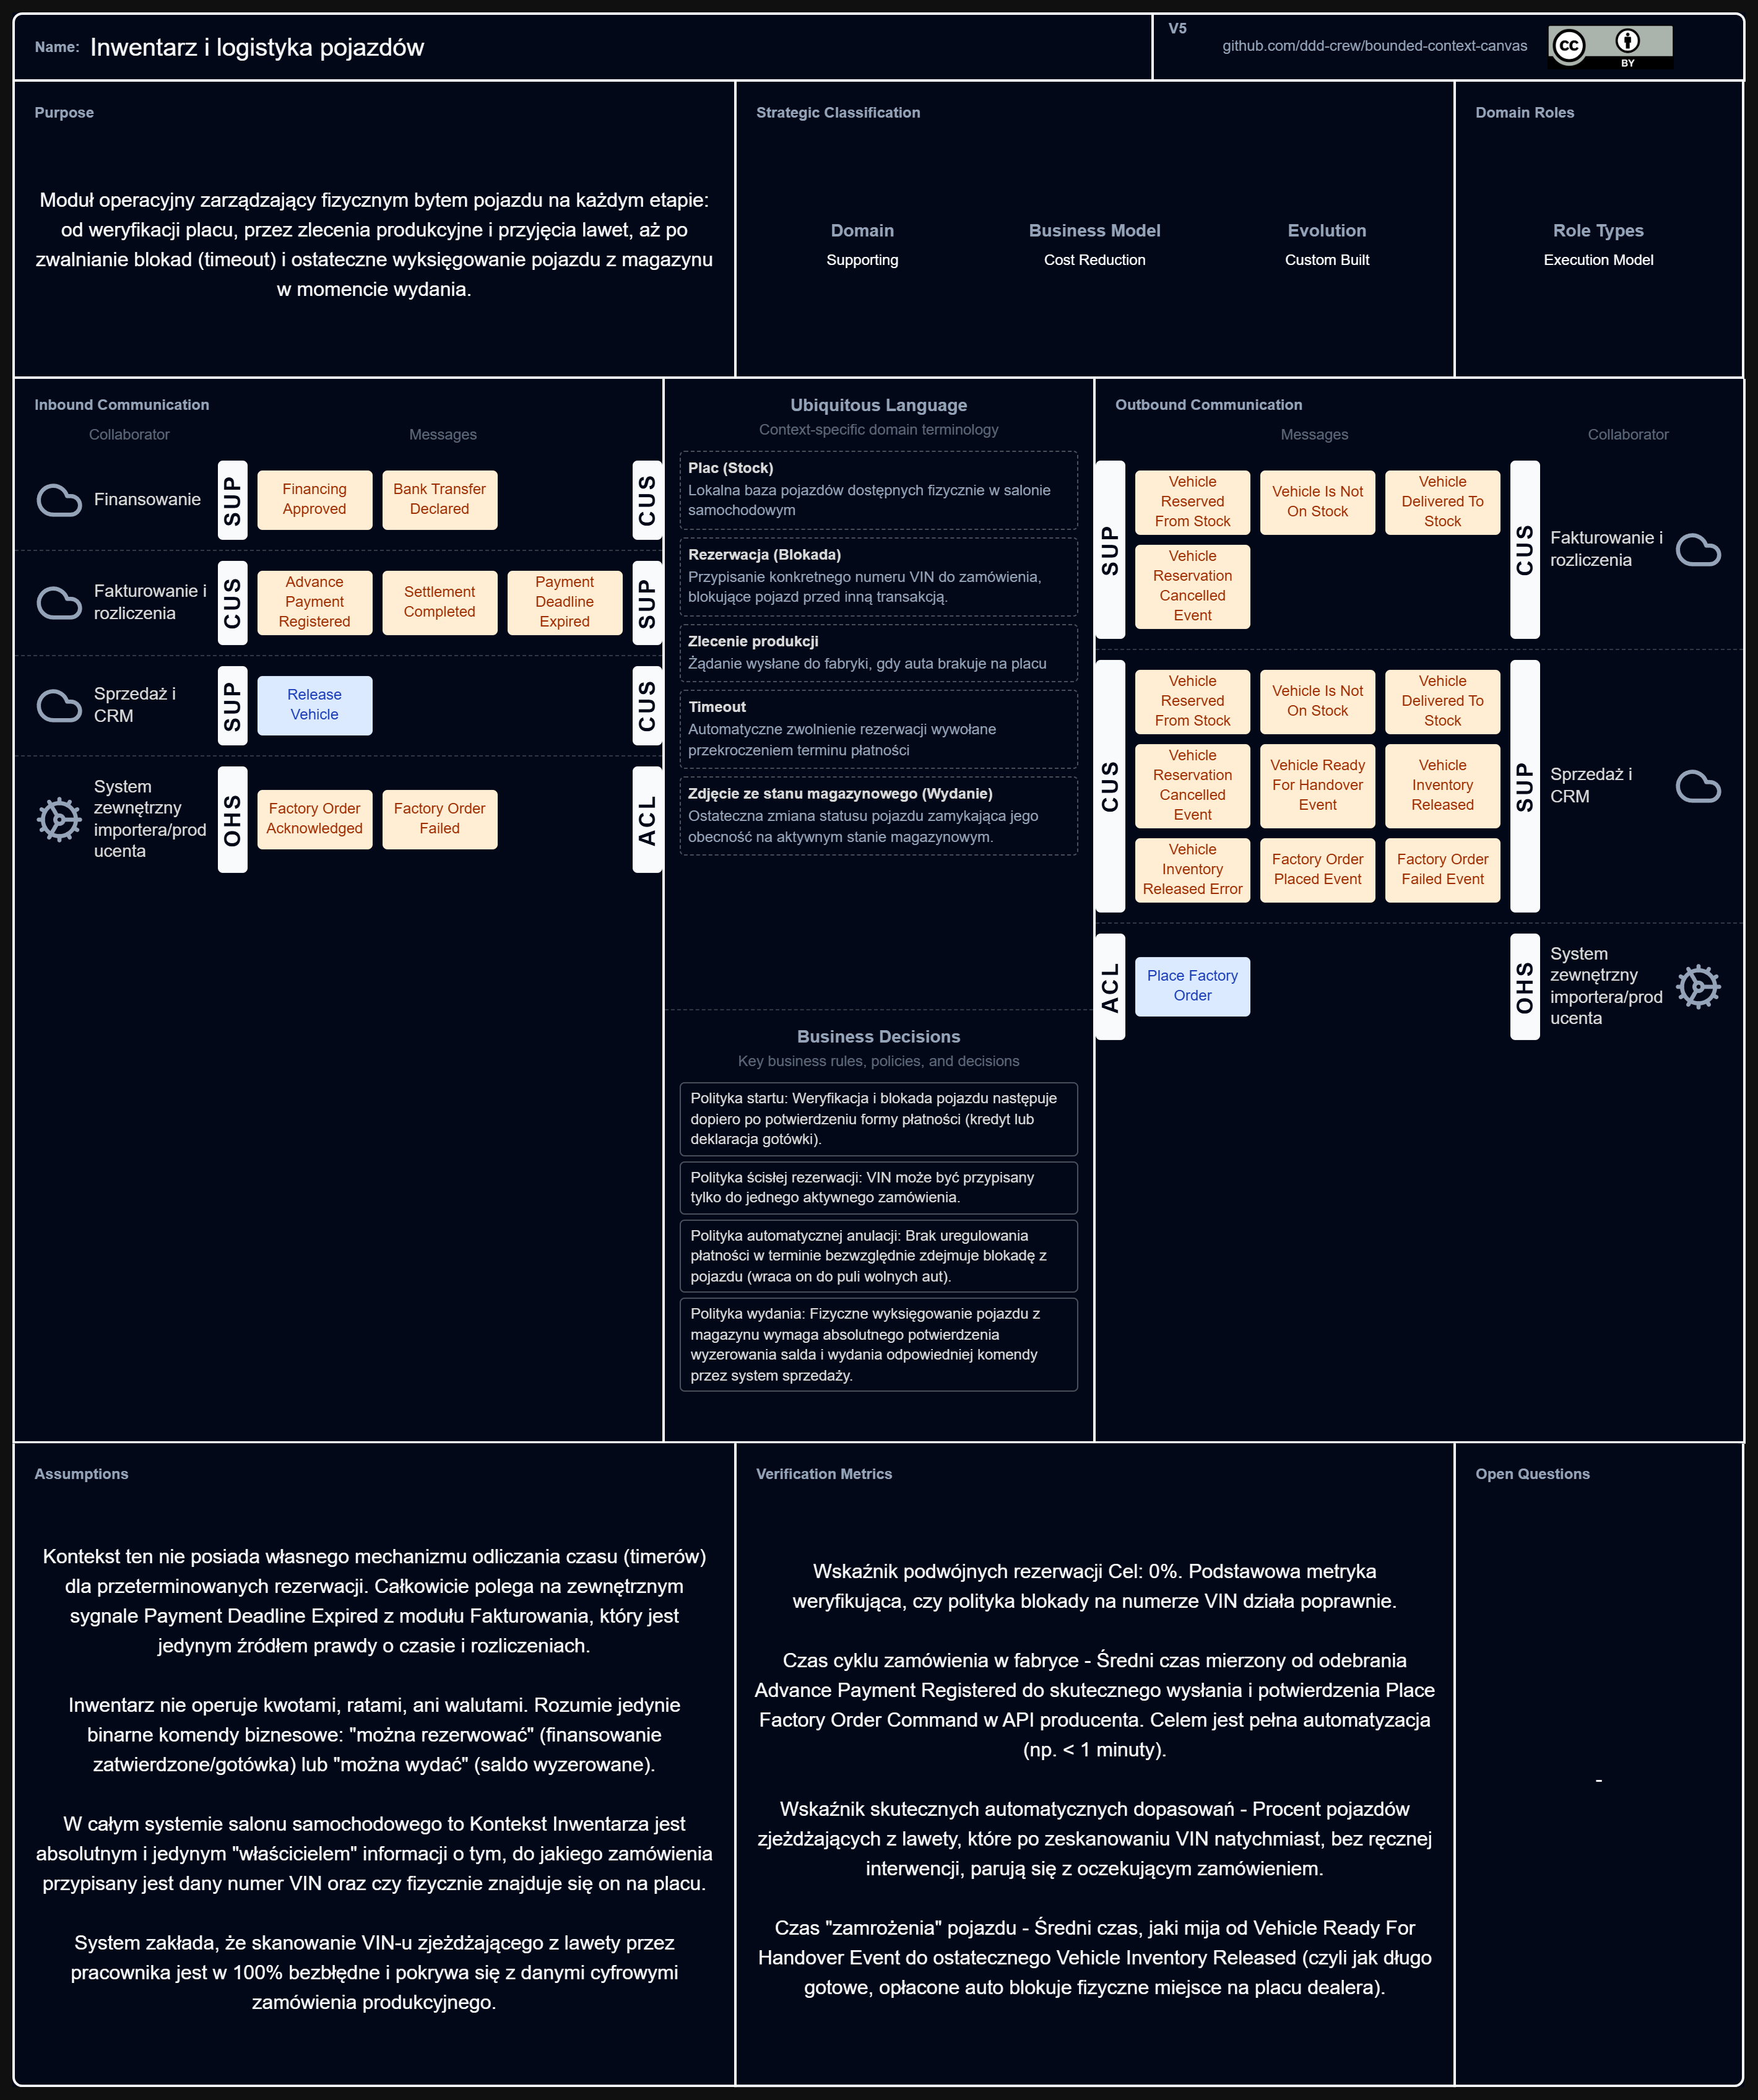
\includegraphics[width=\textwidth]{media/bounded-context-canvas/final/IiLP_K3_TOTAL_FINAL.png}
    \caption{Kanwa Kontekstu  Inwentarza i logistyki pojazdów}
    \label{fig:hex_billing}
\end{figure}
\subsubsection{Przypadki użycia Inwentarza i logistyki pojazdów}

\textbf{UC-INW-01: Weryfikacja dostępności i rezerwacja pojazdu z placu}

\begin{longtable}{|p{4cm}|p{11cm}|}
\hline
\textbf{Element} & \textbf{Opis} \\
\hline

Identyfikator & UC-INW-01 \\
\hline

Nazwa & Weryfikacja dostępności i rezerwacja pojazdu z placu \\
\hline

Opis & 
Sprawdzenie fizycznej dostępności pojazdu o wybranej specyfikacji na placu dealerskim i założenie twardej blokady (rezerwacji) na konkretny numer VIN. \\
\hline

Aktor główny & System (Kontekst Inwentarza i Logistyki) \\
\hline

Aktorzy pomocniczy & - \\
\hline

Warunki wstępne & 
Kontekst otrzymał zdarzenie potwierdzające gotowość do realizacji zamówienia \textit{FinancingApproved} LUB \textit{BankTransferDeclared}. \\
\hline

Warunki końcowe & 
Pojazd zostaje zarezerwowany, system emituje zdarzenie \textit{VehicleReservedFromStock} (dla samochodu na placu) LUB \textit{VehicleNotOnStock} (jeśli nie ma samochodu na stanie magazynowym). \\
\hline

Scenariusz główny & 
\begin{enumerate}
    \item System reaguje na zdarzenie inicjujące proces realizacji.
    \item System przeszukuje lokalną bazę pojazdów dostępnych na placu (status "Wolny") pod kątem specyfikacji z zamówienia.
    \item System znajduje pasujący pojazd i przypisuje jego numer VIN do zamówienia.
    \item System zmienia status pojazdu na "Zarezerwowany".
    \item Kontekst emituje zdarzenie \textit{VehicleReservedFromStockEvent}.
\end{enumerate} \\
\hline

Scenariusze alternatywne & 
\begin{itemize}
    \item [A1] Samochodu nie ma na placu: W kroku 2 system nie znajduje wolnego pojazdu o wymaganej specyfikacji. System wstrzymuje rezerwację i emituje zdarzenie \textit{VehicleNotOnStock}.
\end{itemize} \\
\hline
\end{longtable}

\begin{figure}[H]
    \centering
    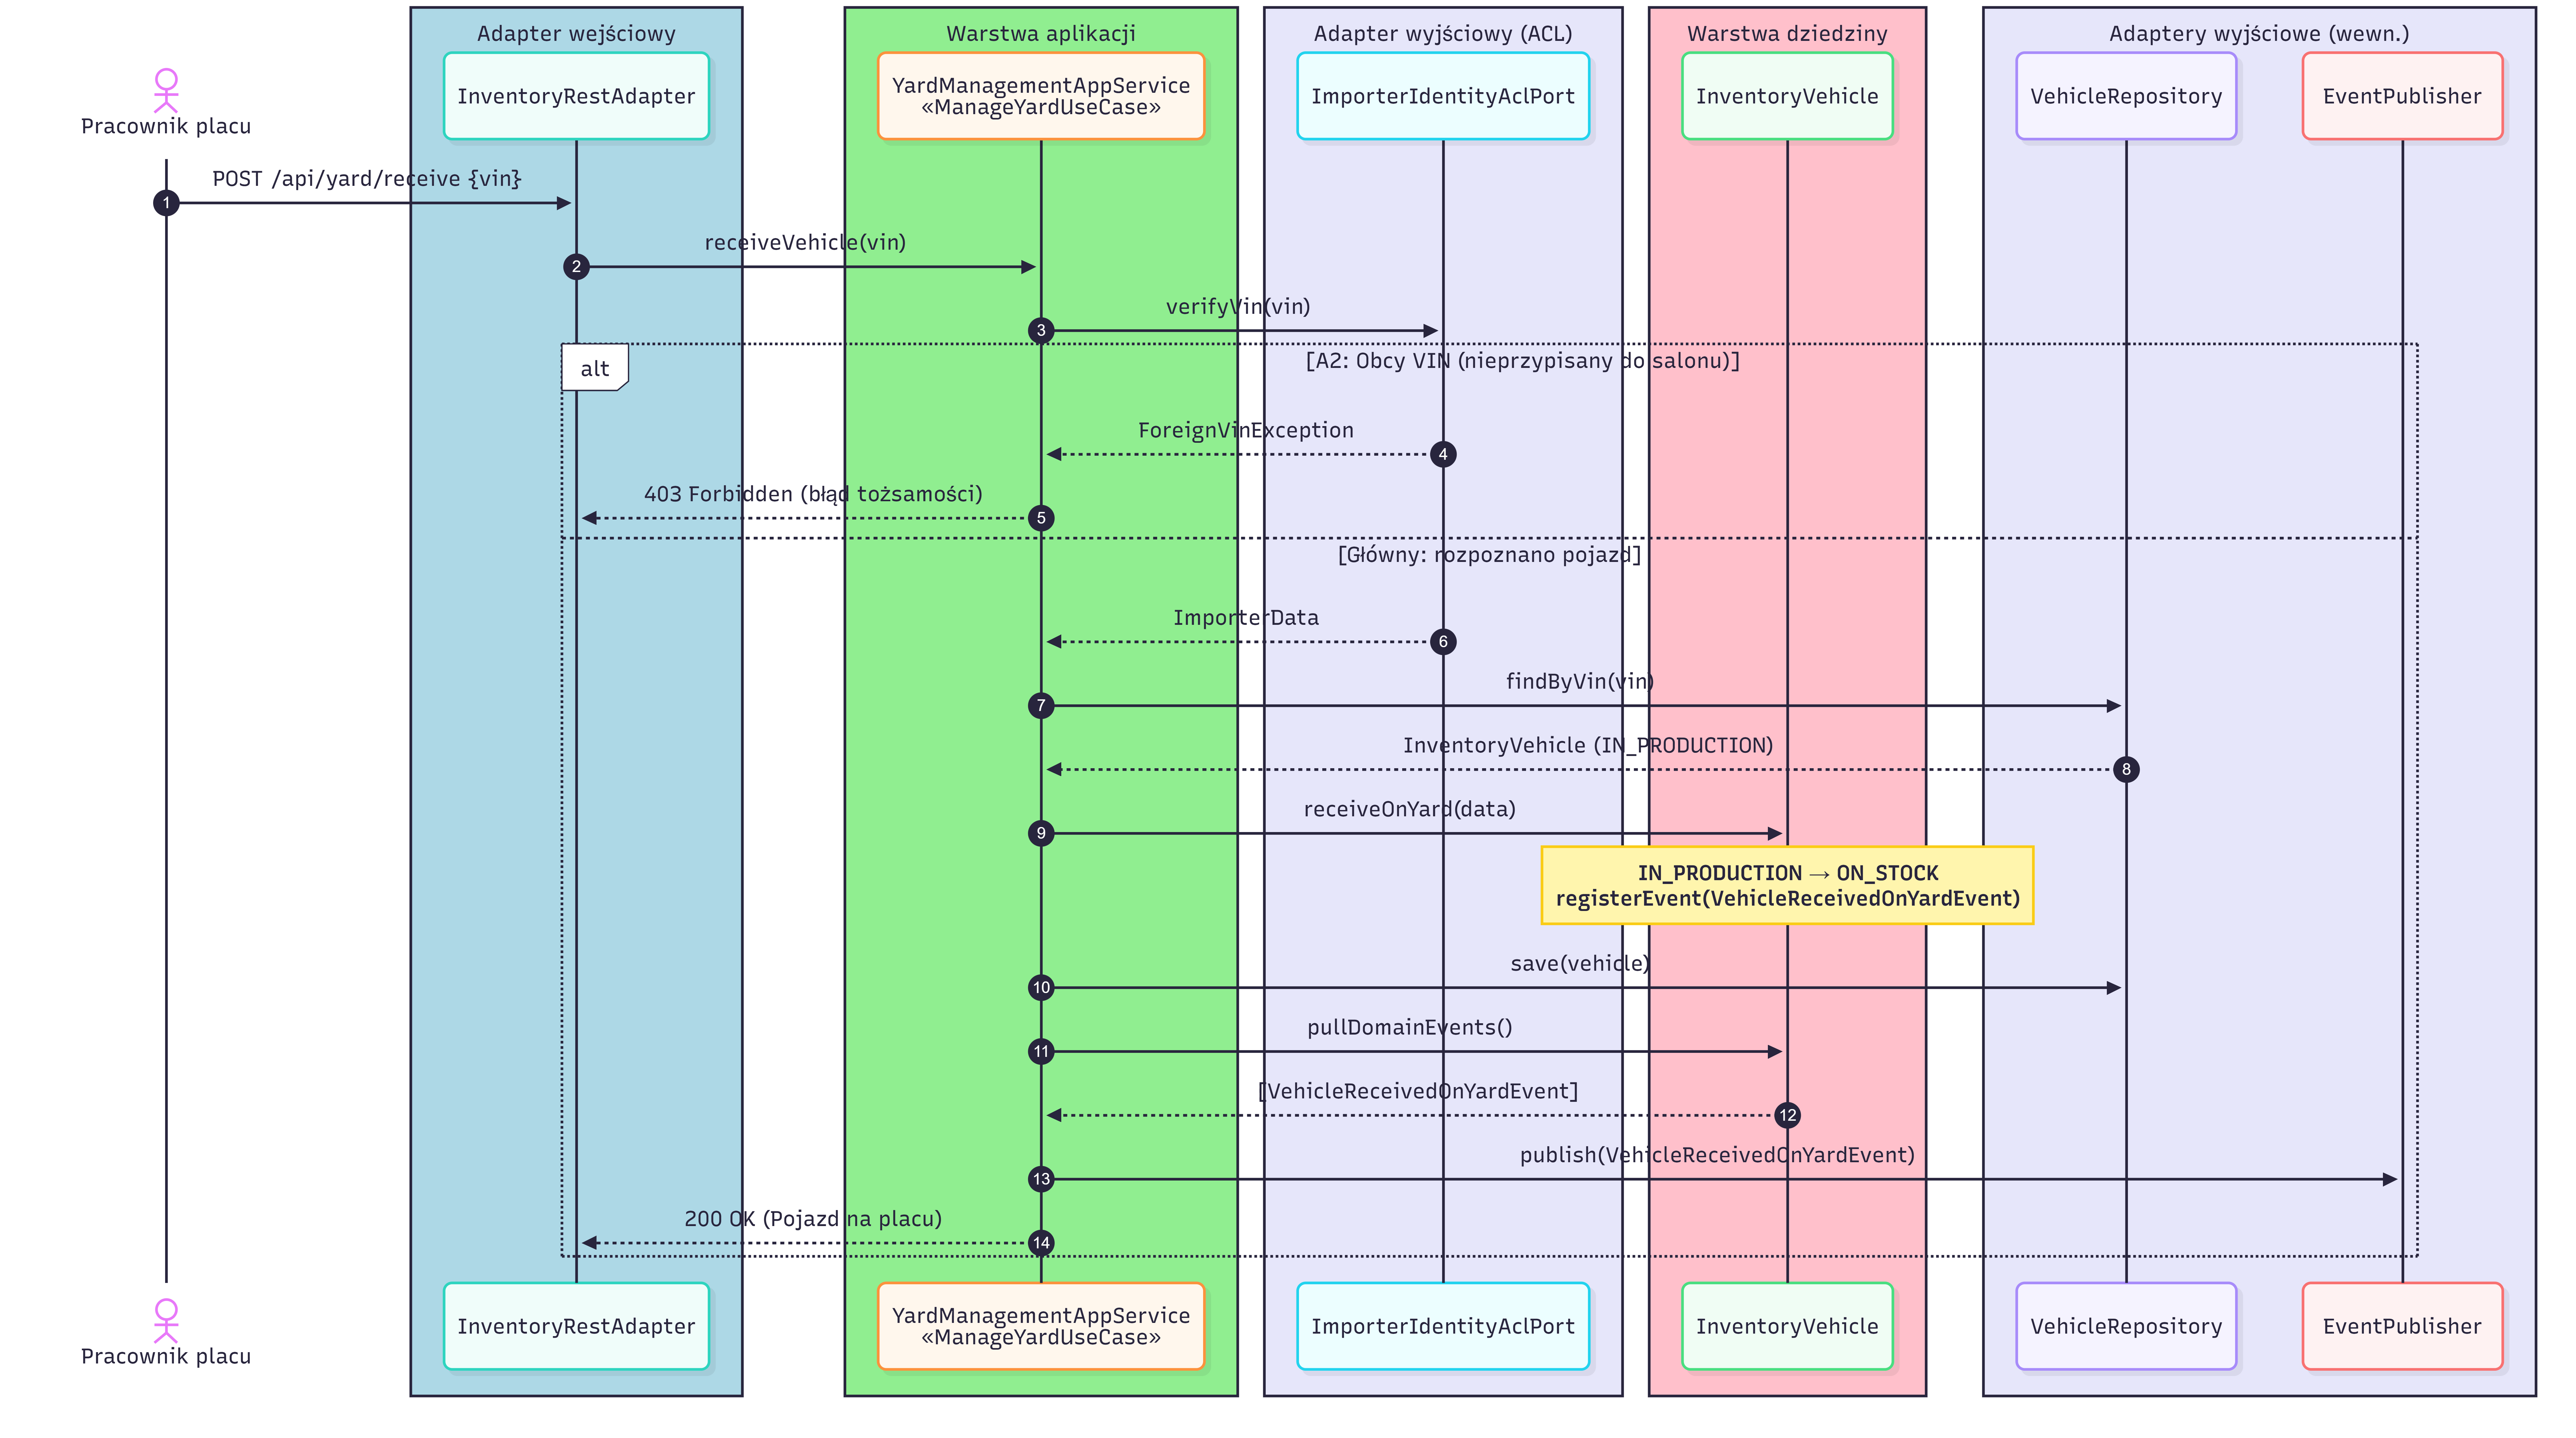
\includegraphics[width=1\textwidth]{media/diagramy_sekwencji/kontekst-inwentarza-logistyki/UC-INW-01-Sekwencji.png}
    \caption{Diagram sekwencji dla przypadku użycia UC-INW-01: Weryfikacja dostępności i rezerwacja pojazdu z placu}
    \label{fig:seq_uc_inw_01}
\end{figure}

% =====================================================
\textbf{UC-INW-02: Zlecenie produkcji pojazdu w fabryce}

\begin{longtable}{|p{4cm}|p{11cm}|}
\hline
\textbf{Element} & \textbf{Opis} \\
\hline

Identyfikator & UC-INW-02 \\
\hline

Nazwa & Zlecenie produkcji pojazdu w fabryce \\
\hline

Opis & 
Zautomatyzowane wysłanie zlecenia produkcji do systemu zewnętrznego fabryki/importera po opłaceniu wymaganego zadatku przez klienta. \\
\hline

Aktor główny & System (Kontekst Inwentarza i Logistyki) \\
\hline

Aktorzy pomocniczy & System zewnętrzny (API Importera) \\
\hline

Warunki wstępne & 
Samochód o określonej specyfikacji nie znajduje się na stanie magazynowym salonu samochodowego. Kontekst otrzymał zdarzenie z \textit{AdvancePaymentRegistered}. \\
\hline

Warunki końcowe & 
Zamówienie produkcyjne zostaje wysłane, a system emituje zdarzenie \textit{FactoryOrderPlacedEvent}. \\
\hline

Scenariusz główny & 
\begin{enumerate}
    \item System reaguje na zdarzenie o opłaceniu zadatku.
    \item System generuje żądanie produkcyjne na podstawie zatwierdzonej specyfikacji.
    \item System komunikuje się z API Importera/Fabryki i wysyła zlecenie.
    \item System oznacza to zamówienie lokalnie statusem "W produkcji".
    \item Kontekst emituje zdarzenie \textit{FactoryOrderPlacedEvent}.
\end{enumerate} \\
\hline

Scenariusze alternatywne & 
\begin{itemize}
    \item [A1] Fabryka odrzuca zlecenie: W kroku 3 API fabryki zwraca błąd (np. problem z połączeniem). System emituje zdarzenie \textit{FactoryOrderFailed}.
\end{itemize} \\
\hline
\end{longtable}

\begin{figure}[H]
    \centering
    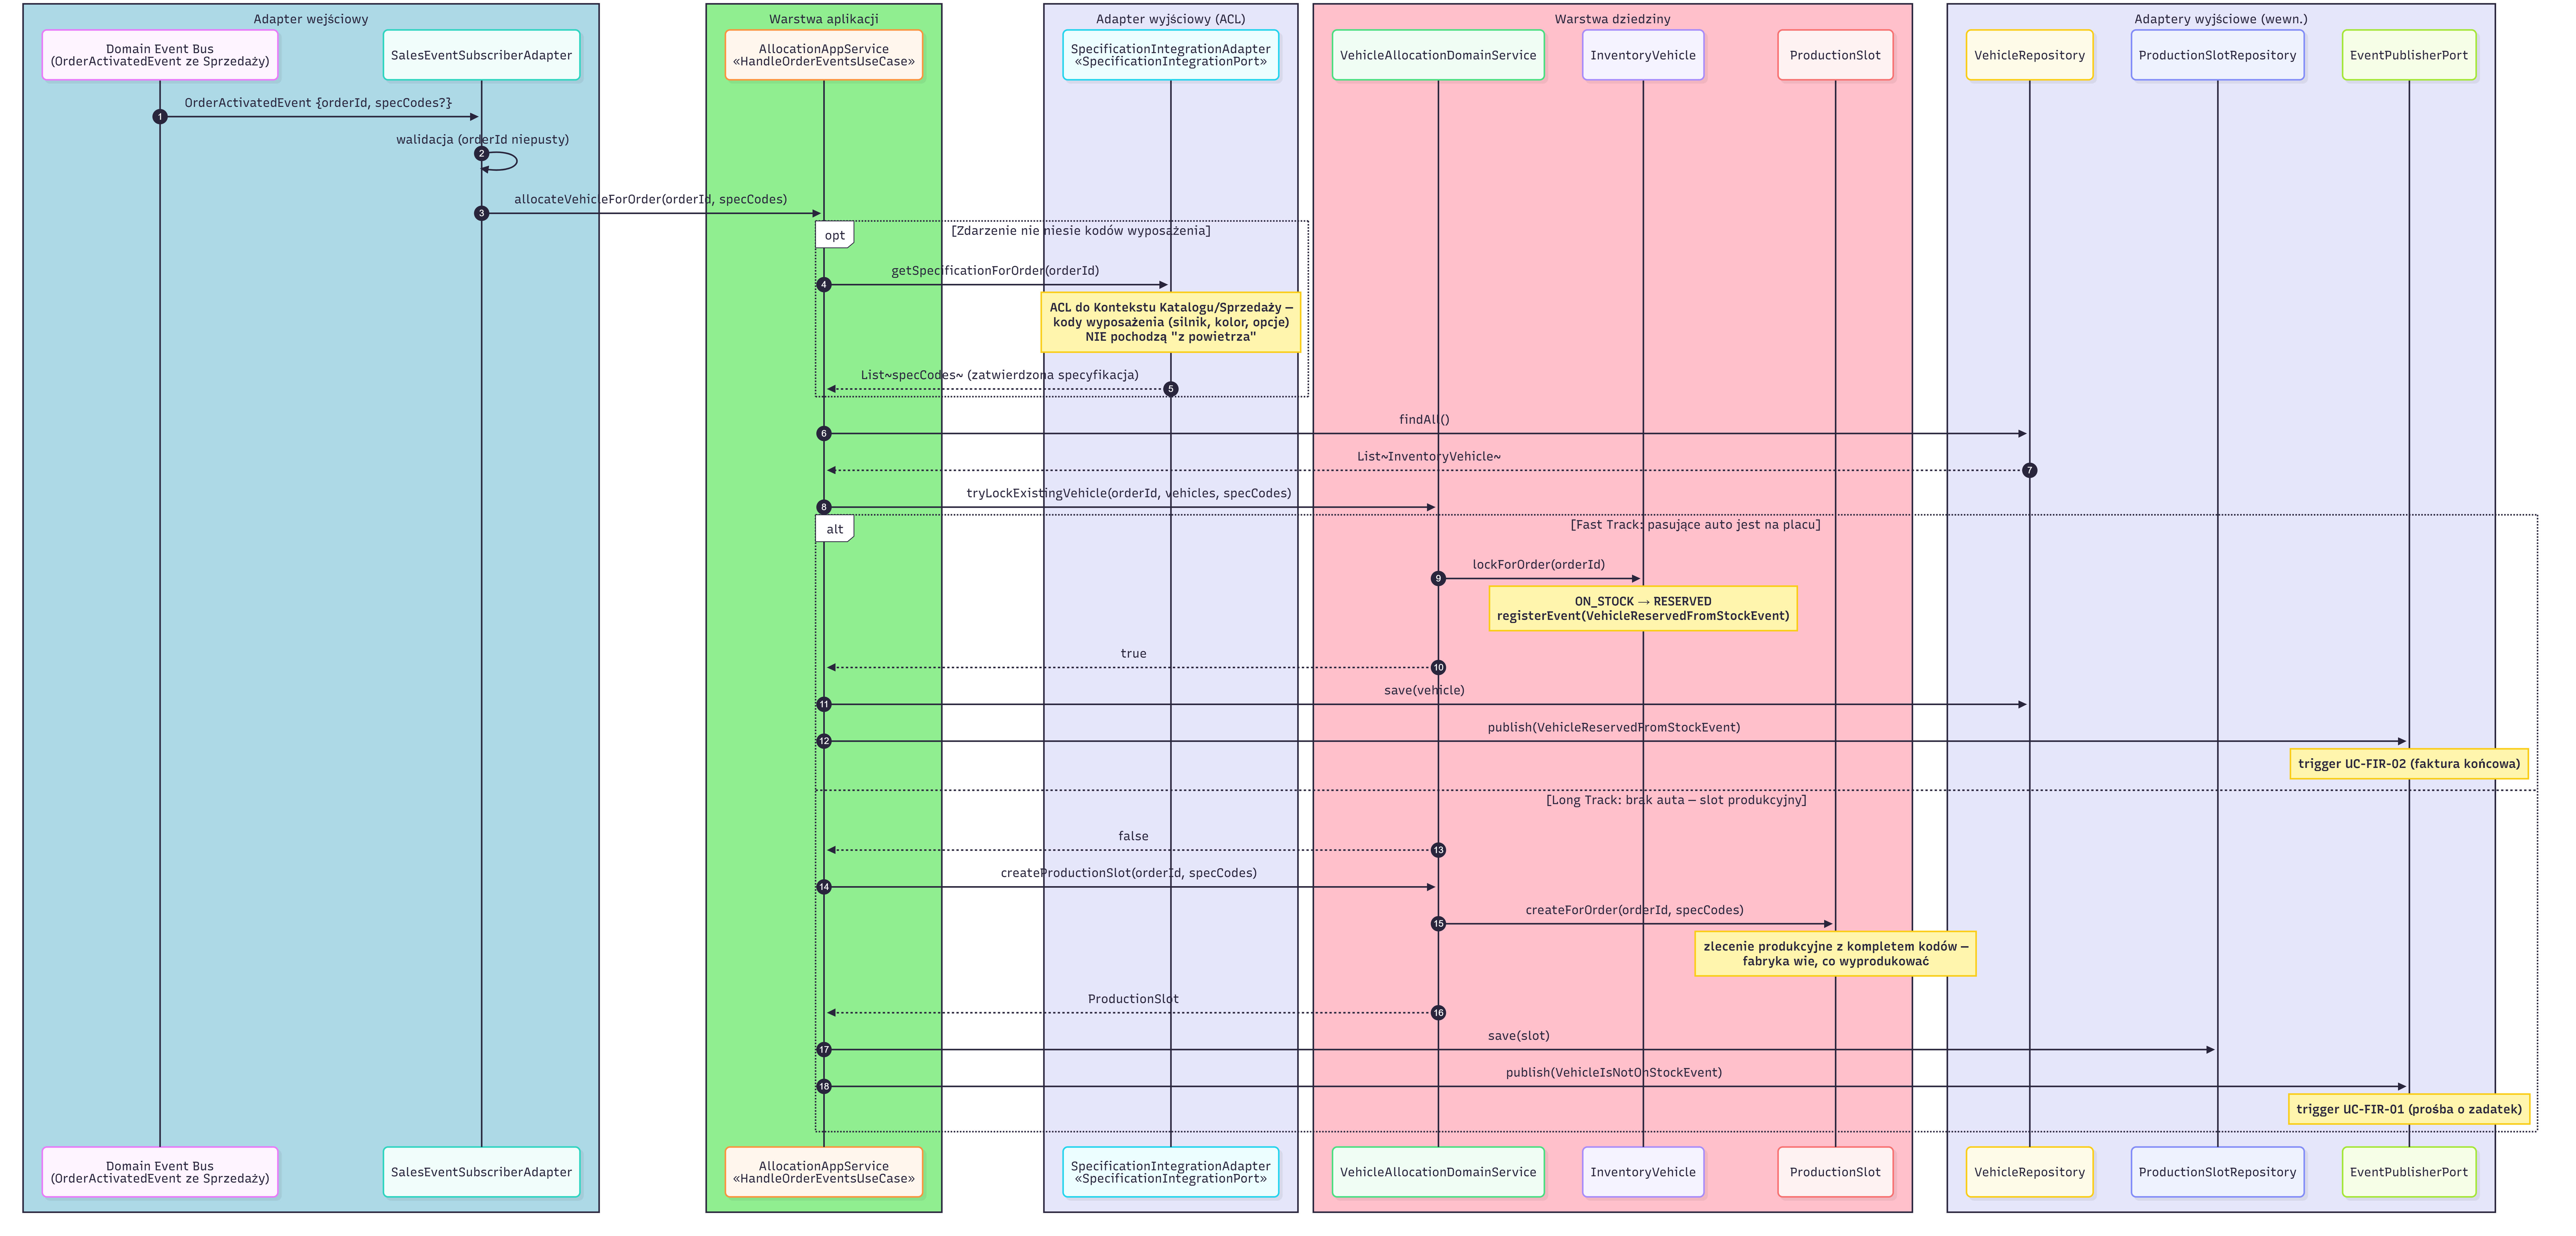
\includegraphics[width=1\textwidth]{media/diagramy_sekwencji/kontekst-inwentarza-logistyki/UC-INW-02-Sekwencji.png}
    \caption{Diagram sekwencji dla przypadku użycia UC-INW-02: Zlecenie produkcji pojazdu w fabryce}
    \label{fig:seq_uc_inw_02}
\end{figure}

% =====================================================
\textbf{UC-INW-03: Przyjęcie pojazdu na stan magazynowy}

\begin{longtable}{|p{4cm}|p{11cm}|}
\hline
\textbf{Element} & \textbf{Opis} \\
\hline

Identyfikator & UC-INW-03 \\
\hline

Nazwa & Przyjęcie pojazdu na stan magazynowy \\
\hline

Opis & 
Rejestracja fizycznego pojazdu, który przyjechał z fabryki na plac dealera, oraz powiązanie jego numeru VIN z oczekującym zamówieniem. \\
\hline

Aktor główny & Pracownik Placu (lub System Logistyczny Importera) \\
\hline

Aktorzy pomocniczy & - \\
\hline

Warunki wstępne & 
Fizyczny pojazd dotarł na plac salonu samochodowego. W systemie istnieje zamówienie o statusie "W produkcji". \\
\hline

Warunki końcowe & 
Pojazd jest zarejestrowany na stanie, otrzymuje status "Zarezerwowany" (przypisany do klienta), a system emituje zdarzenie \textit{VehicleDeliveredToStock}. \\
\hline

Scenariusz główny & 
\begin{enumerate}
    \item Pracownik placu rejestruje zjazd auta z lawety (skanując VIN).
    \item System tworzy nową kartotekę pojazdu w lokalnym inwentarzu.
    \item System automatycznie paruje ten numer VIN z oczekującym zamówieniem klienta.
    \item System zmienia status pojazdu na "Zarezerwowany".
    \item Kontekst emituje zdarzenie \textit{VehicleDeliveredToStock}.
\end{enumerate} \\
\hline

Scenariusze alternatywne & 
\begin{itemize}
    \item [A1] Auto nieprzypisane: W kroku 3 system nie znajduje zamówienia dla danej specyfikacji (np. auto zamówione "na stock"). Pojazd otrzymuje status "Wolny". Zdarzenie końcowe \textit{VehicleDeliveredToStock} nie jest emitowane.
\end{itemize} \\
\hline
\end{longtable}

\begin{figure}[H]
    \centering
    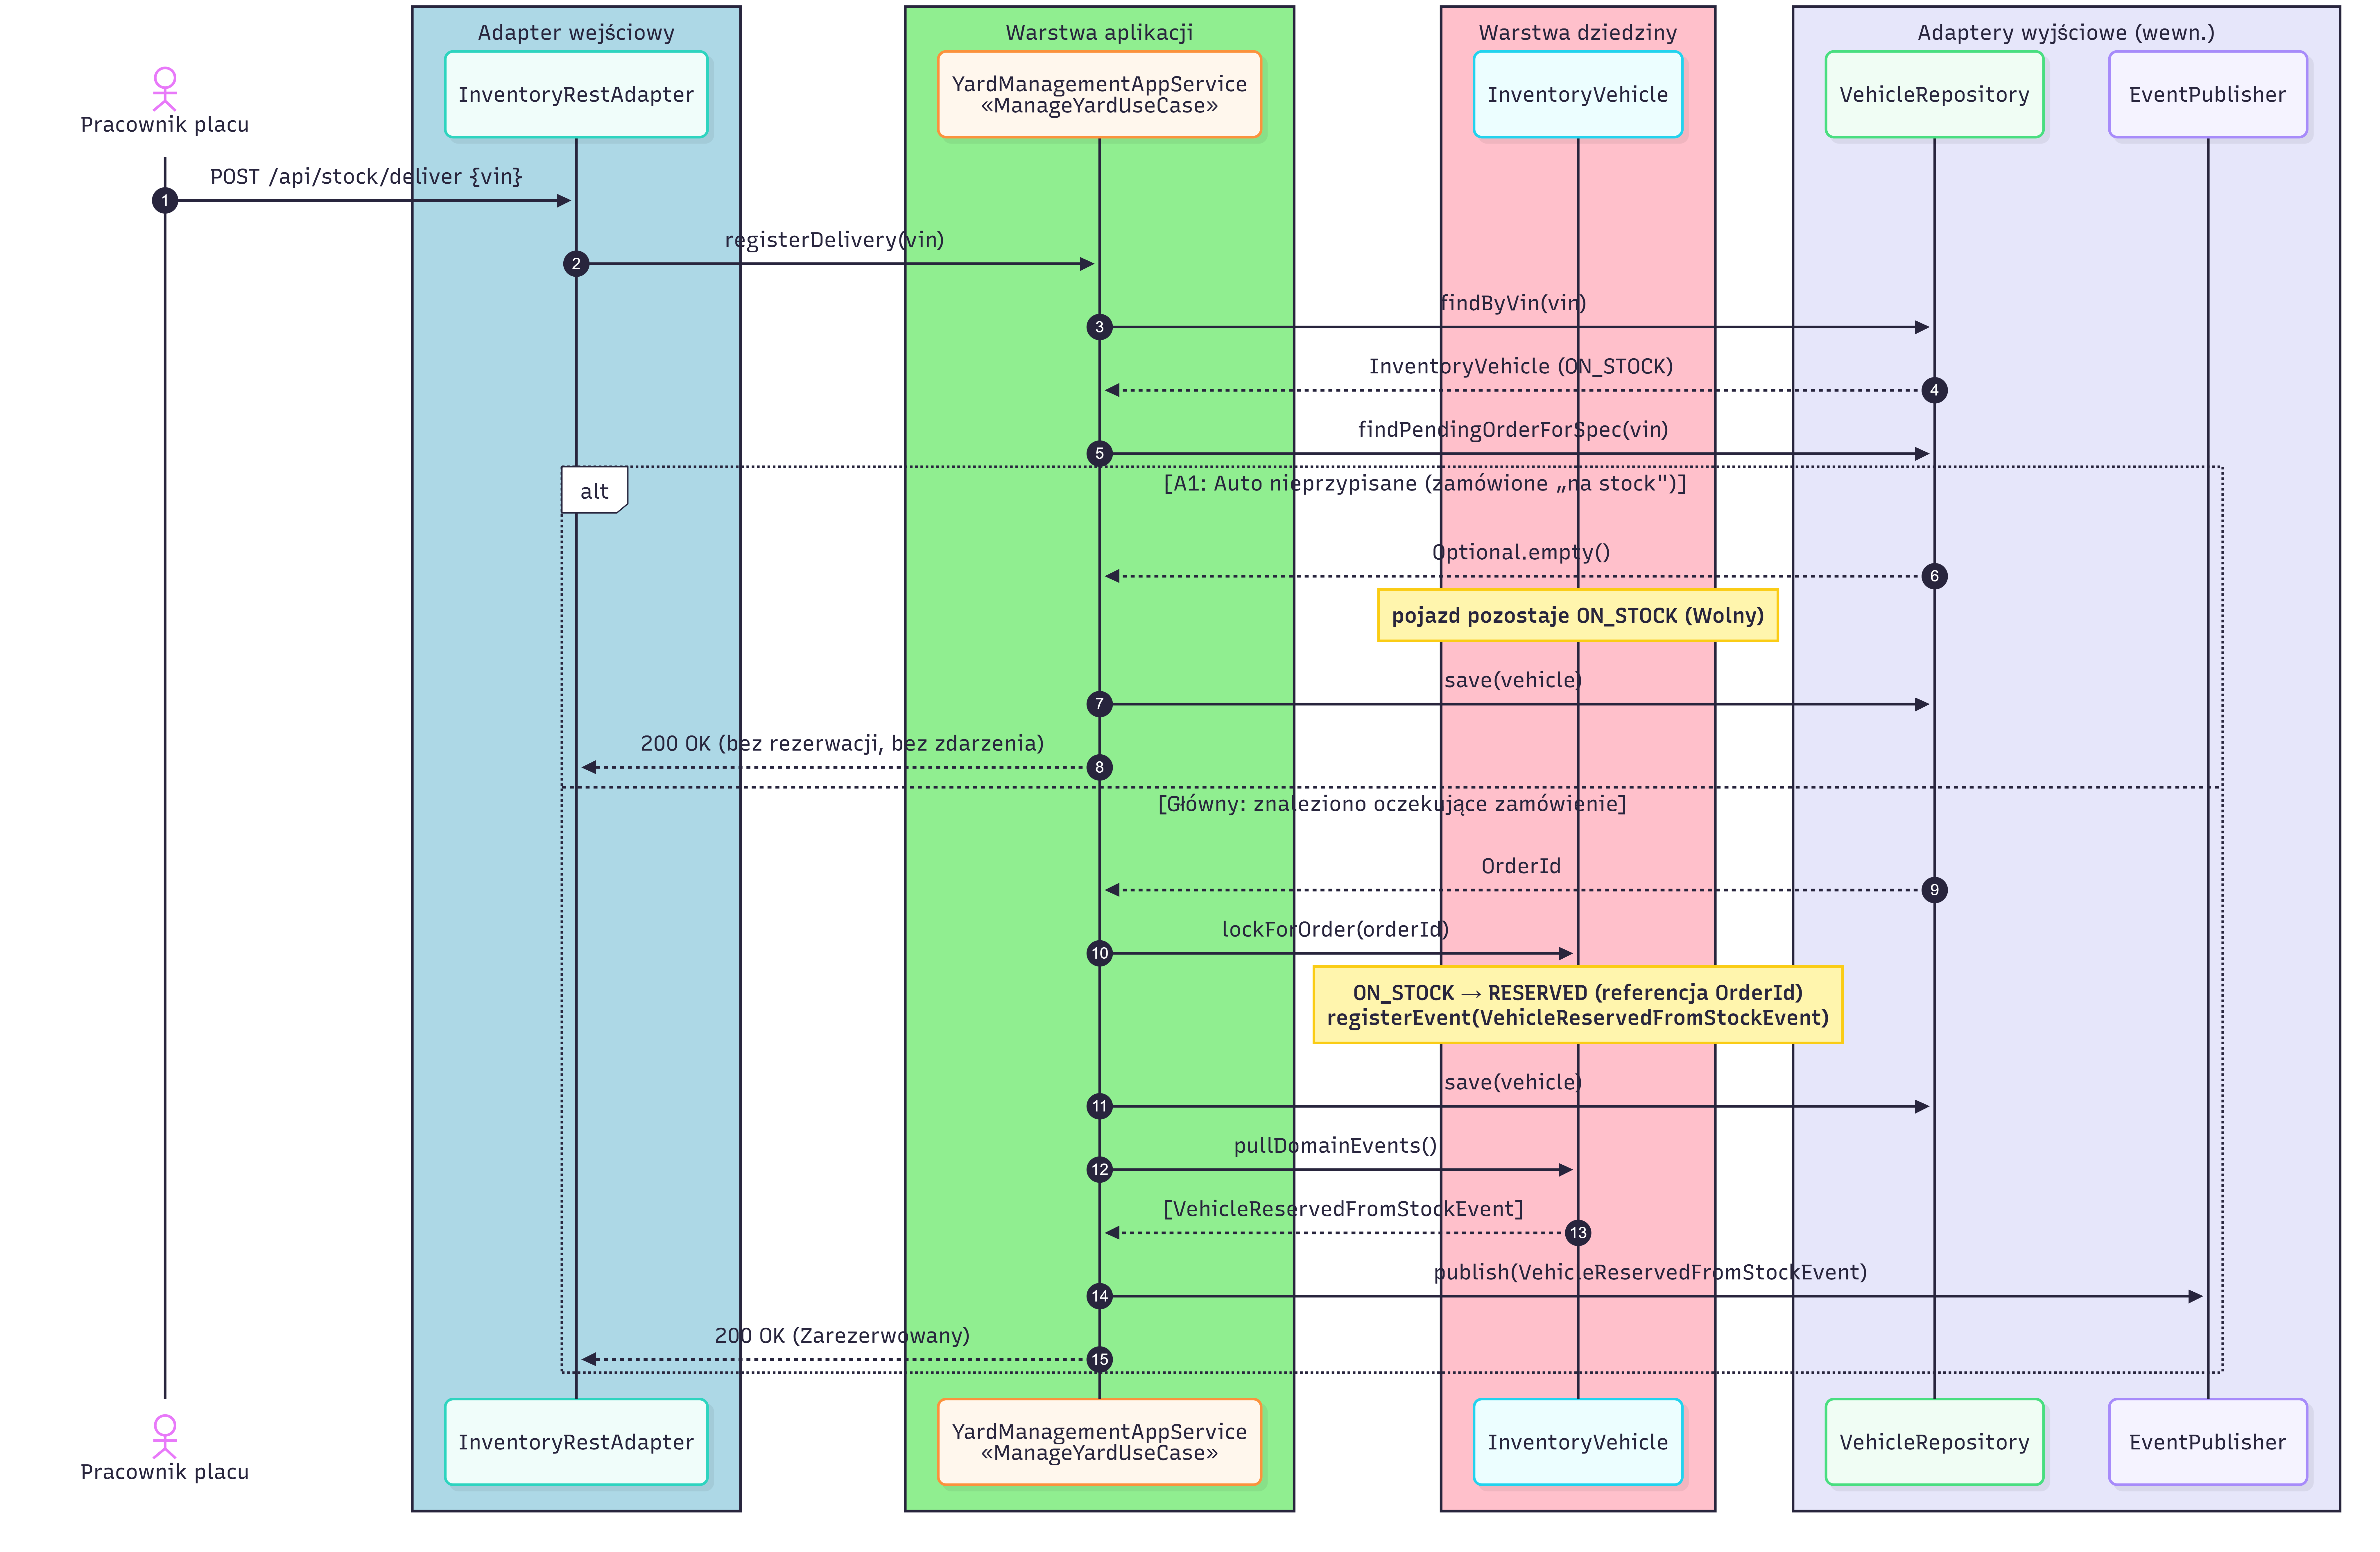
\includegraphics[width=1\textwidth]{media/diagramy_sekwencji/kontekst-inwentarza-logistyki/UC-INW-03-Sekwencji.png}
    \caption{Diagram sekwencji dla przypadku użycia UC-INW-03: Przyjęcie pojazdu na stan magazynowy}
    \label{fig:seq_uc_inw_03}
\end{figure}

% =====================================================
\textbf{UC-INW-04: Zwolnienie blokady pojazdu}

\begin{longtable}{|p{4cm}|p{11cm}|}
\hline
\textbf{Element} & \textbf{Opis} \\
\hline

Identyfikator & UC-INW-04 \\
\hline

Nazwa & Zwolnienie blokady pojazdu \\
\hline

Opis & 
Automatyczne zdjęcie rezerwacji z numeru VIN w przypadku braku uregulowania płatności końcowej w wyznaczonym terminie. \\
\hline

Aktor główny & System (Kontekst Inwentarza i Logistyki) \\
\hline

Aktorzy pomocniczy & - \\
\hline

Warunki wstępne & 
Kontekst otrzymał zdarzenie \textit{PaymentDeadlineExpired}. \\
\hline

Warunki końcowe & 
Pojazd wraca na plac do ponownej sprzedaży, emitowane jest zdarzenie \textit{VehicleReservationCancelledEvent}. \\
\hline

Scenariusz główny & 
\begin{enumerate}
    \item System reaguje na zdarzenie \textit{PaymentDeadlineExpired}.
    \item System wyszukuje numer VIN zablokowany dla tego zamówienia.
    \item System usuwa powiązanie VIN z zamówieniem i zmienia status pojazdu na "Wolny".
    \item Kontekst emituje zdarzenie \textit{VehicleReservationCancelledEvent}.
\end{enumerate} \\
\hline

Scenariusze alternatywne & 
\begin{itemize}
    \item [A1] Pojazd nie istnieje w rezerwacjach: Zablokowany pojazd został wcześniej usunięty/wydany.
\end{itemize} \\
\hline
\end{longtable}

\begin{figure}[H]
    \centering
    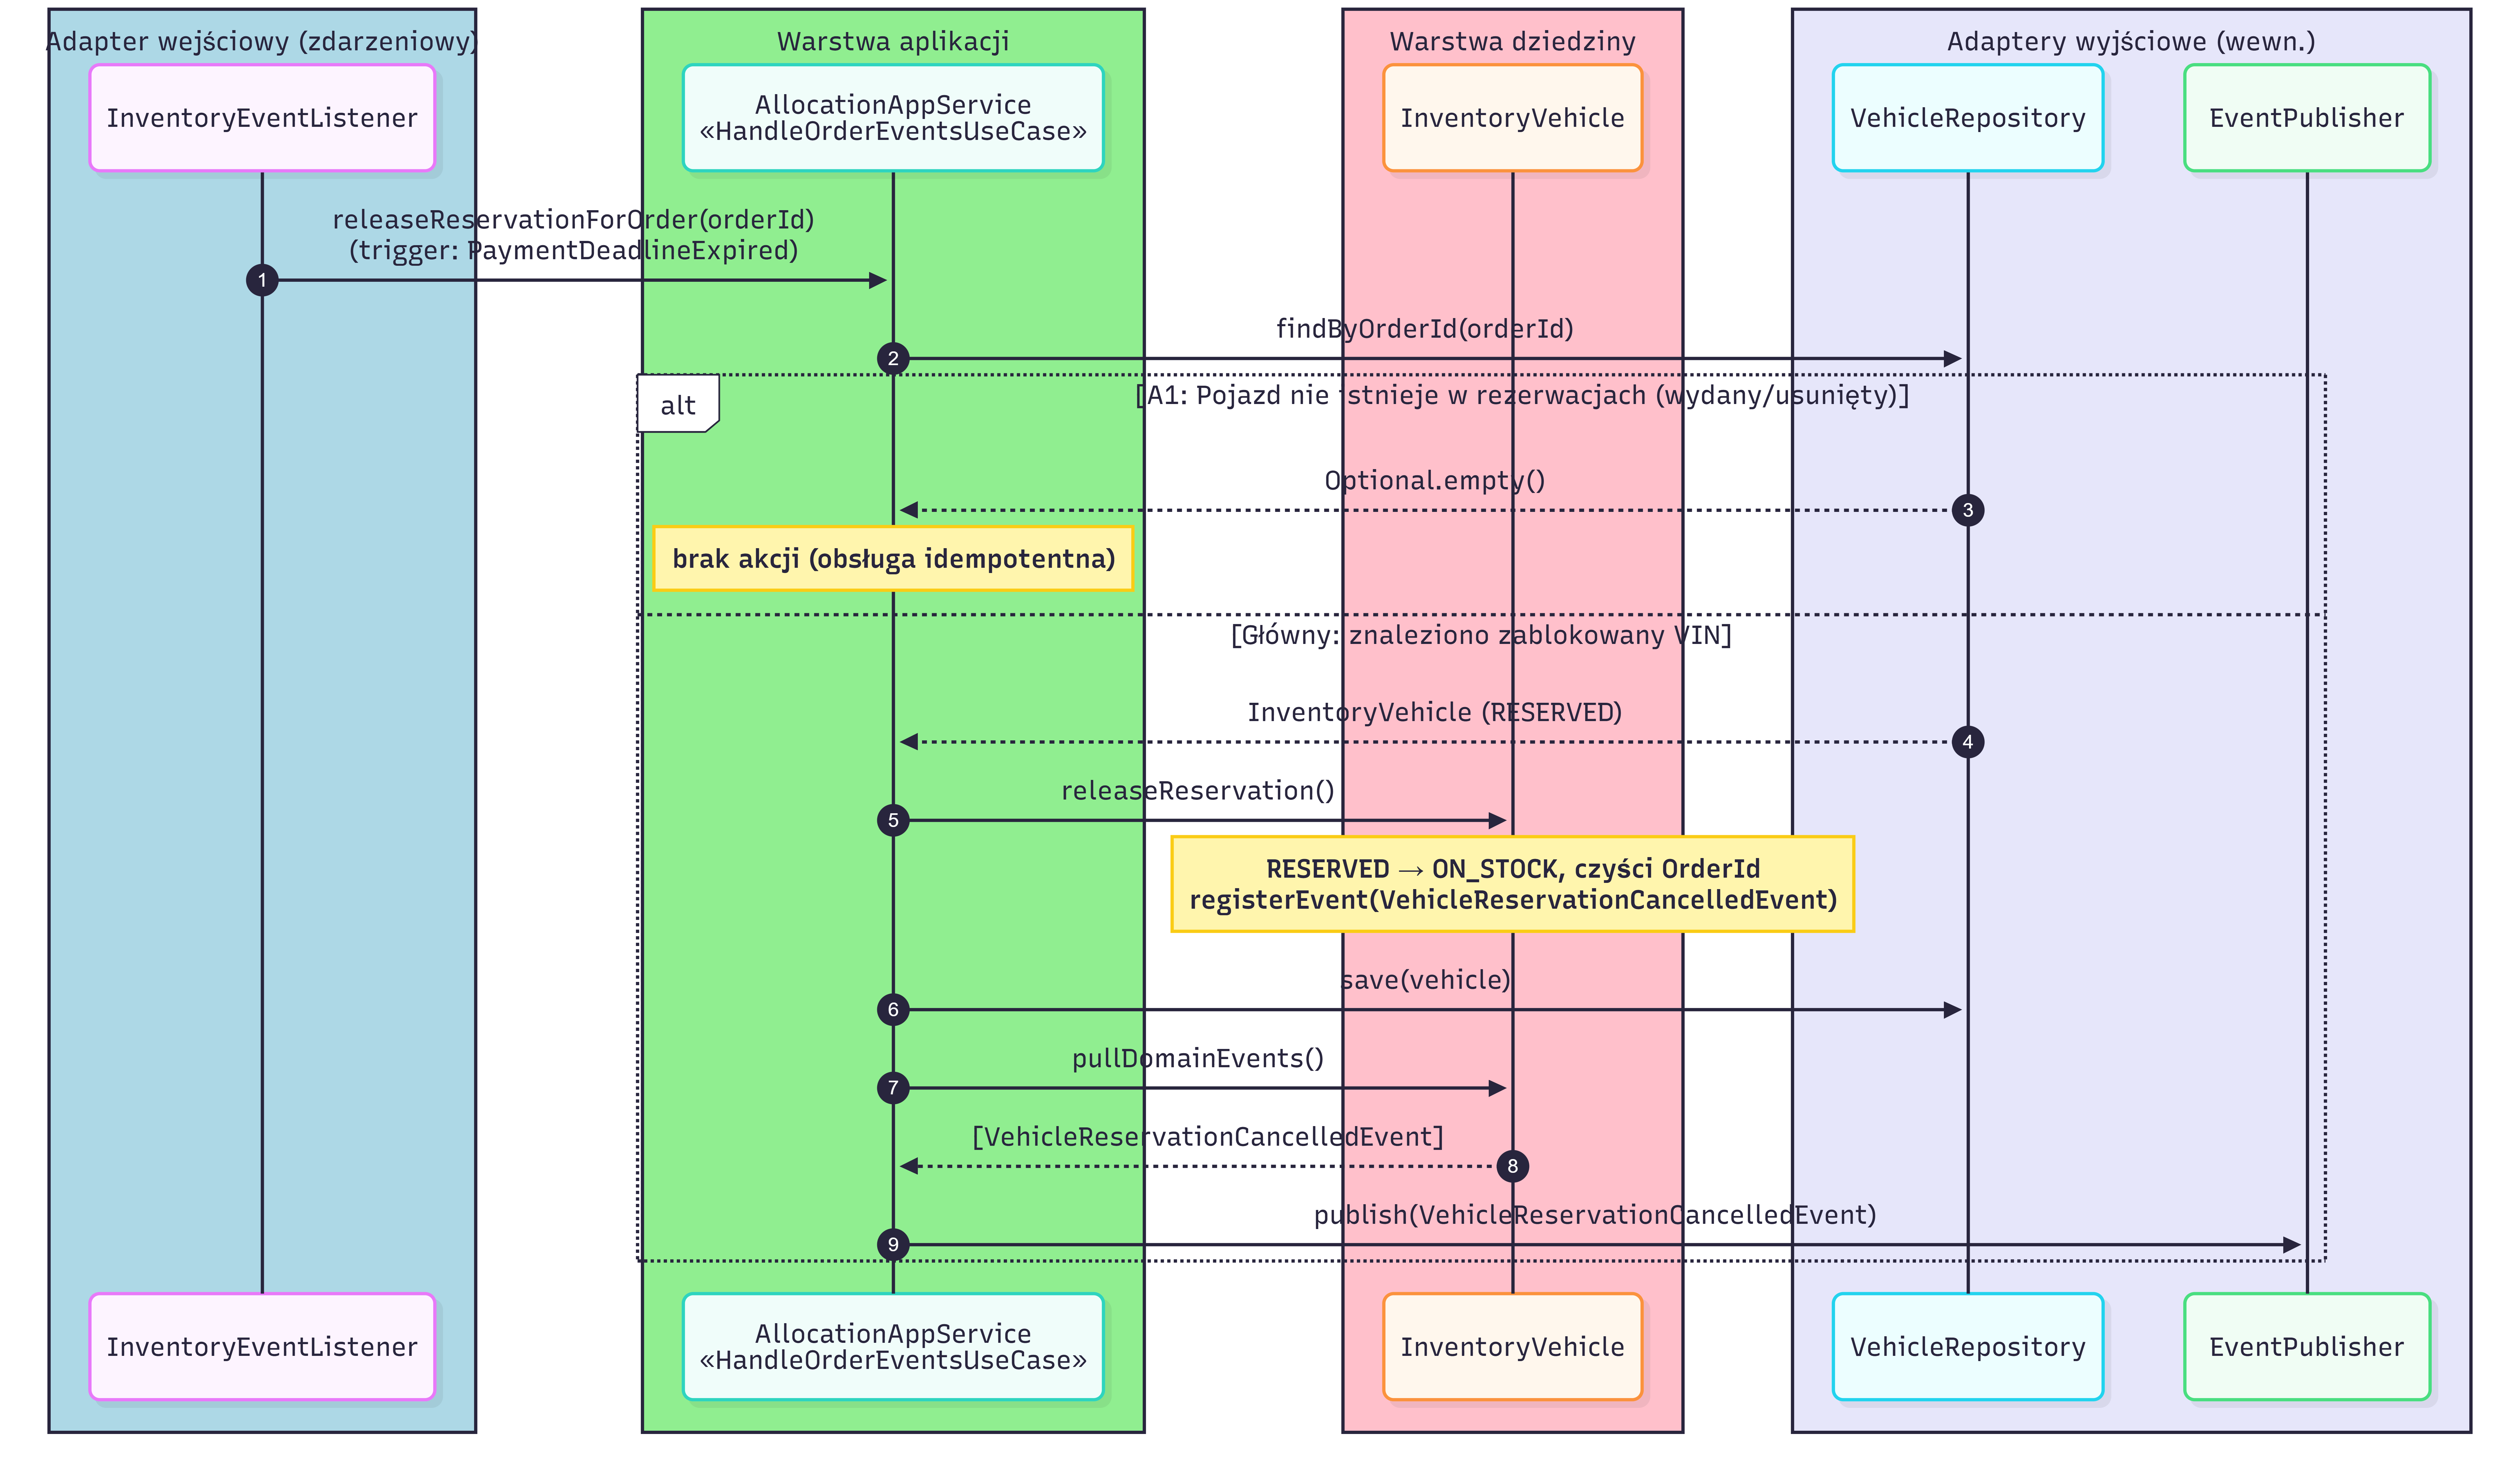
\includegraphics[width=1\textwidth]{media/diagramy_sekwencji/kontekst-inwentarza-logistyki/UC-INW-04-Sekwencji.png}
    \caption{Diagram sekwencji dla przypadku użycia UC-INW-04: Zwolnienie blokady pojazdu}
    \label{fig:seq_uc_inw_04}
\end{figure}

% =====================================================
\textbf{UC-INW-05: Przygotowanie pojazdu do wydania po rozliczeniu}

\begin{longtable}{|p{4cm}|p{11cm}|}
\hline
\textbf{Element} & \textbf{Opis} \\
\hline

Identyfikator & UC-INW-05 \\
\hline

Nazwa & Przygotowanie pojazdu do wydania po rozliczeniu \\
\hline

Opis & 
Systemowa zmiana statusu pojazdu na "Gotowy do wydania" po otrzymaniu potwierdzenia pełnego rozliczenia zamówienia. \\
\hline

Aktor główny & System (Kontekst Inwentarza) \\
\hline

Aktorzy pomocniczy & - \\
\hline

Warunki wstępne & 
Pojazd ma status 'Zarezerwowany', kontekst otrzymał zdarzenie \textit{SettlementCompleted}. \\
\hline

Warunki końcowe & 
Status pojazdu zmieniony na 'Gotowy do wydania', emitowane zdarzenie \textit{VehicleReadyForHandover}. \\
\hline

Scenariusz główny & 
\begin{enumerate}
    \item System reaguje na zdarzenie \textit{SettlementCompleted}.
    \item System weryfikuje, czy dla danego VIN-u istnieje aktywna rezerwacja.
    \item System zmienia status pojazdu z 'Zarezerwowany' na 'Gotowy do wydania'.
    \item Kontekst emituje zdarzenie \textit{VehicleReadyForHandoverEvent}.
\end{enumerate} \\
\hline

Scenariusze alternatywne & 
\begin{itemize}
    \item [] Brak.
\end{itemize} \\
\hline
\end{longtable}

\begin{figure}[H]
    \centering
    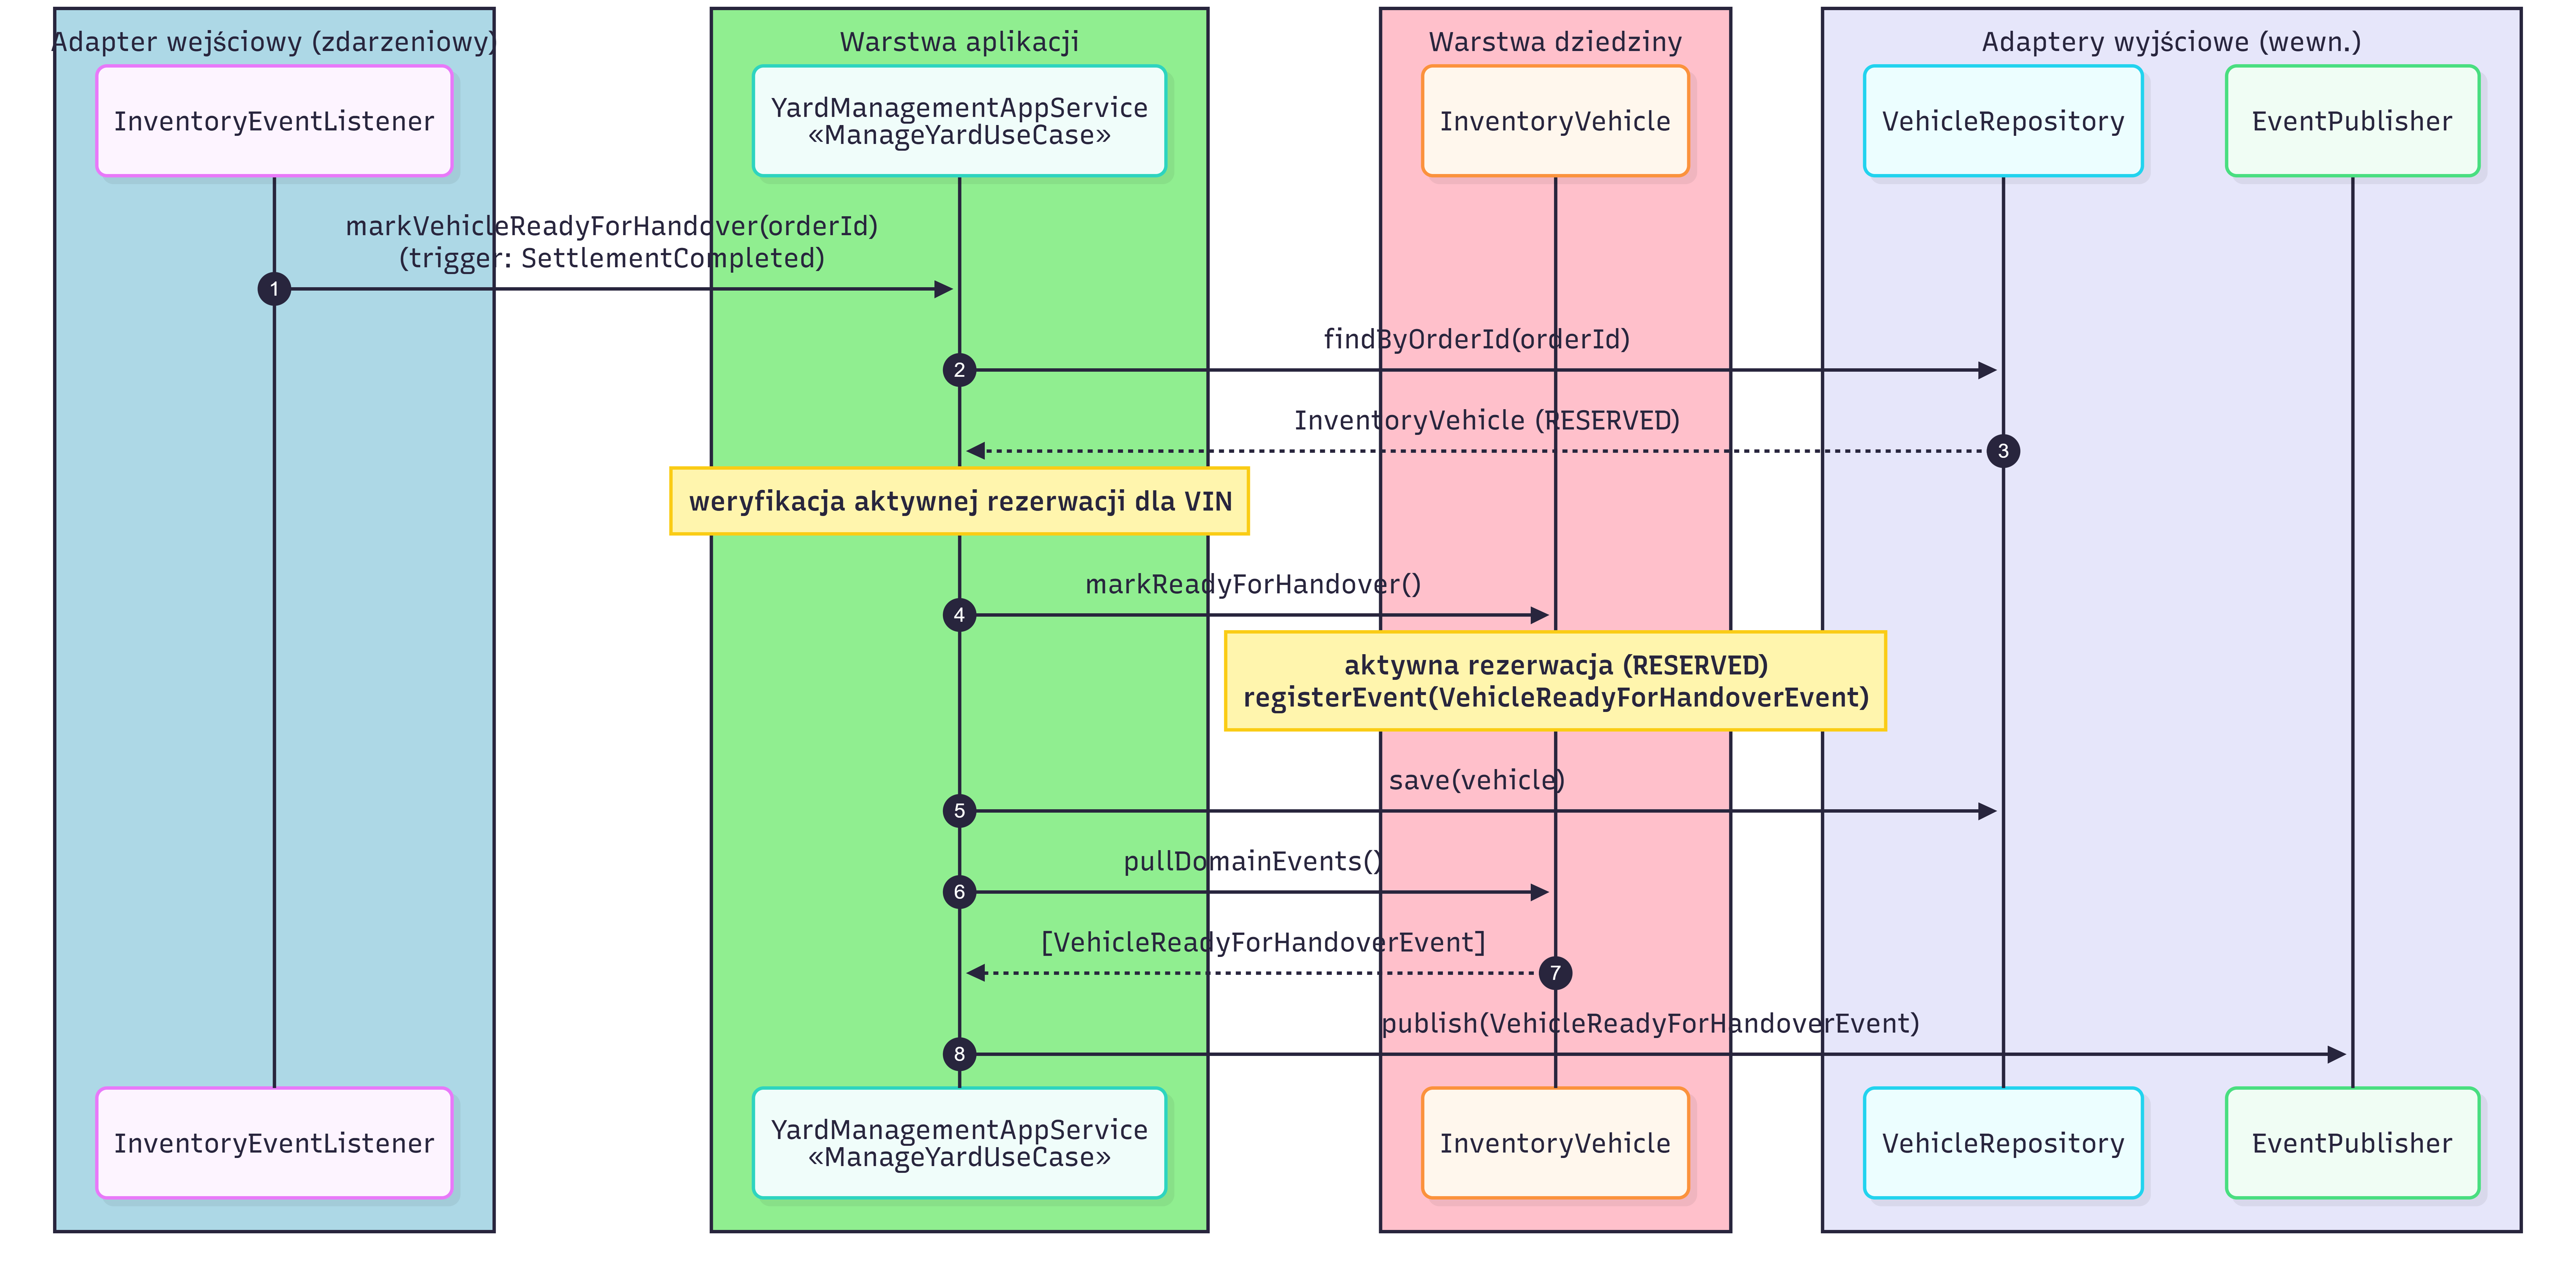
\includegraphics[width=1\textwidth]{media/diagramy_sekwencji/kontekst-inwentarza-logistyki/UC-INW-05-Sekwencji.png}
    \caption{Diagram sekwencji dla przypadku użycia UC-INW-05: Przygotowanie pojazdu do wydania po rozliczeniu}
    \label{fig:seq_uc_inw_05}
\end{figure}

% =====================================================
\textbf{UC-INW-06: Zdjęcie pojazdu ze stanu magazynowego}

\begin{longtable}{|p{4cm}|p{11cm}|}
\hline
\textbf{Element} & \textbf{Opis} \\
\hline

Identyfikator & UC-INW-06 \\
\hline

Nazwa & Zdjęcie pojazdu ze stanu magazynowego \\
\hline

Opis & 
Automatyczna operacja zmiany statusu pojazdu na "Wydany" w Inwentarzu, wywołana komendą z modułu Sprzedaży/CRM. \\
\hline

Aktor główny & System (Kontekst Inwentarza i Logistyki) \\
\hline

Aktorzy pomocniczy & - \\
\hline

Warunki wstępne & 
Pojazd ma status "Gotowy do wydania". Kontekst otrzymał komendę oznaczającą fizyczne wydanie auta \textit{ReleaseVehicle}. \\
\hline

Warunki końcowe & 
Status pojazdu zmieniony na "Wydany", emitowane zdarzenie \textit{VehicleInventoryReleased}. \\
\hline

Scenariusz główny & 
\begin{enumerate}
    \item System Inwentarza odbiera komendę \textit{ReleaseVehicle}.
    \item System weryfikuje status pojazdu pod kątem gotowości do wydania.
    \item System zdejmuje pojazd z aktywnego stanu magazynowego, zmieniając jego status na "Wydany".
    \item Kontekst emituje zdarzenie \textit{VehicleInventoryReleased}.
\end{enumerate} \\
\hline

Scenariusze alternatywne & 
\begin{itemize}
    \item [A1] Niewłaściwy status pojazdu: W kroku 2 pojazd ma status inny niż "Gotowy do wydania". System odrzuca komendę i emituje zdarzenie \textit{VehicleInventoryReleasedError}.
\end{itemize} \\
\hline
\end{longtable}

\begin{figure}[H]
    \centering
    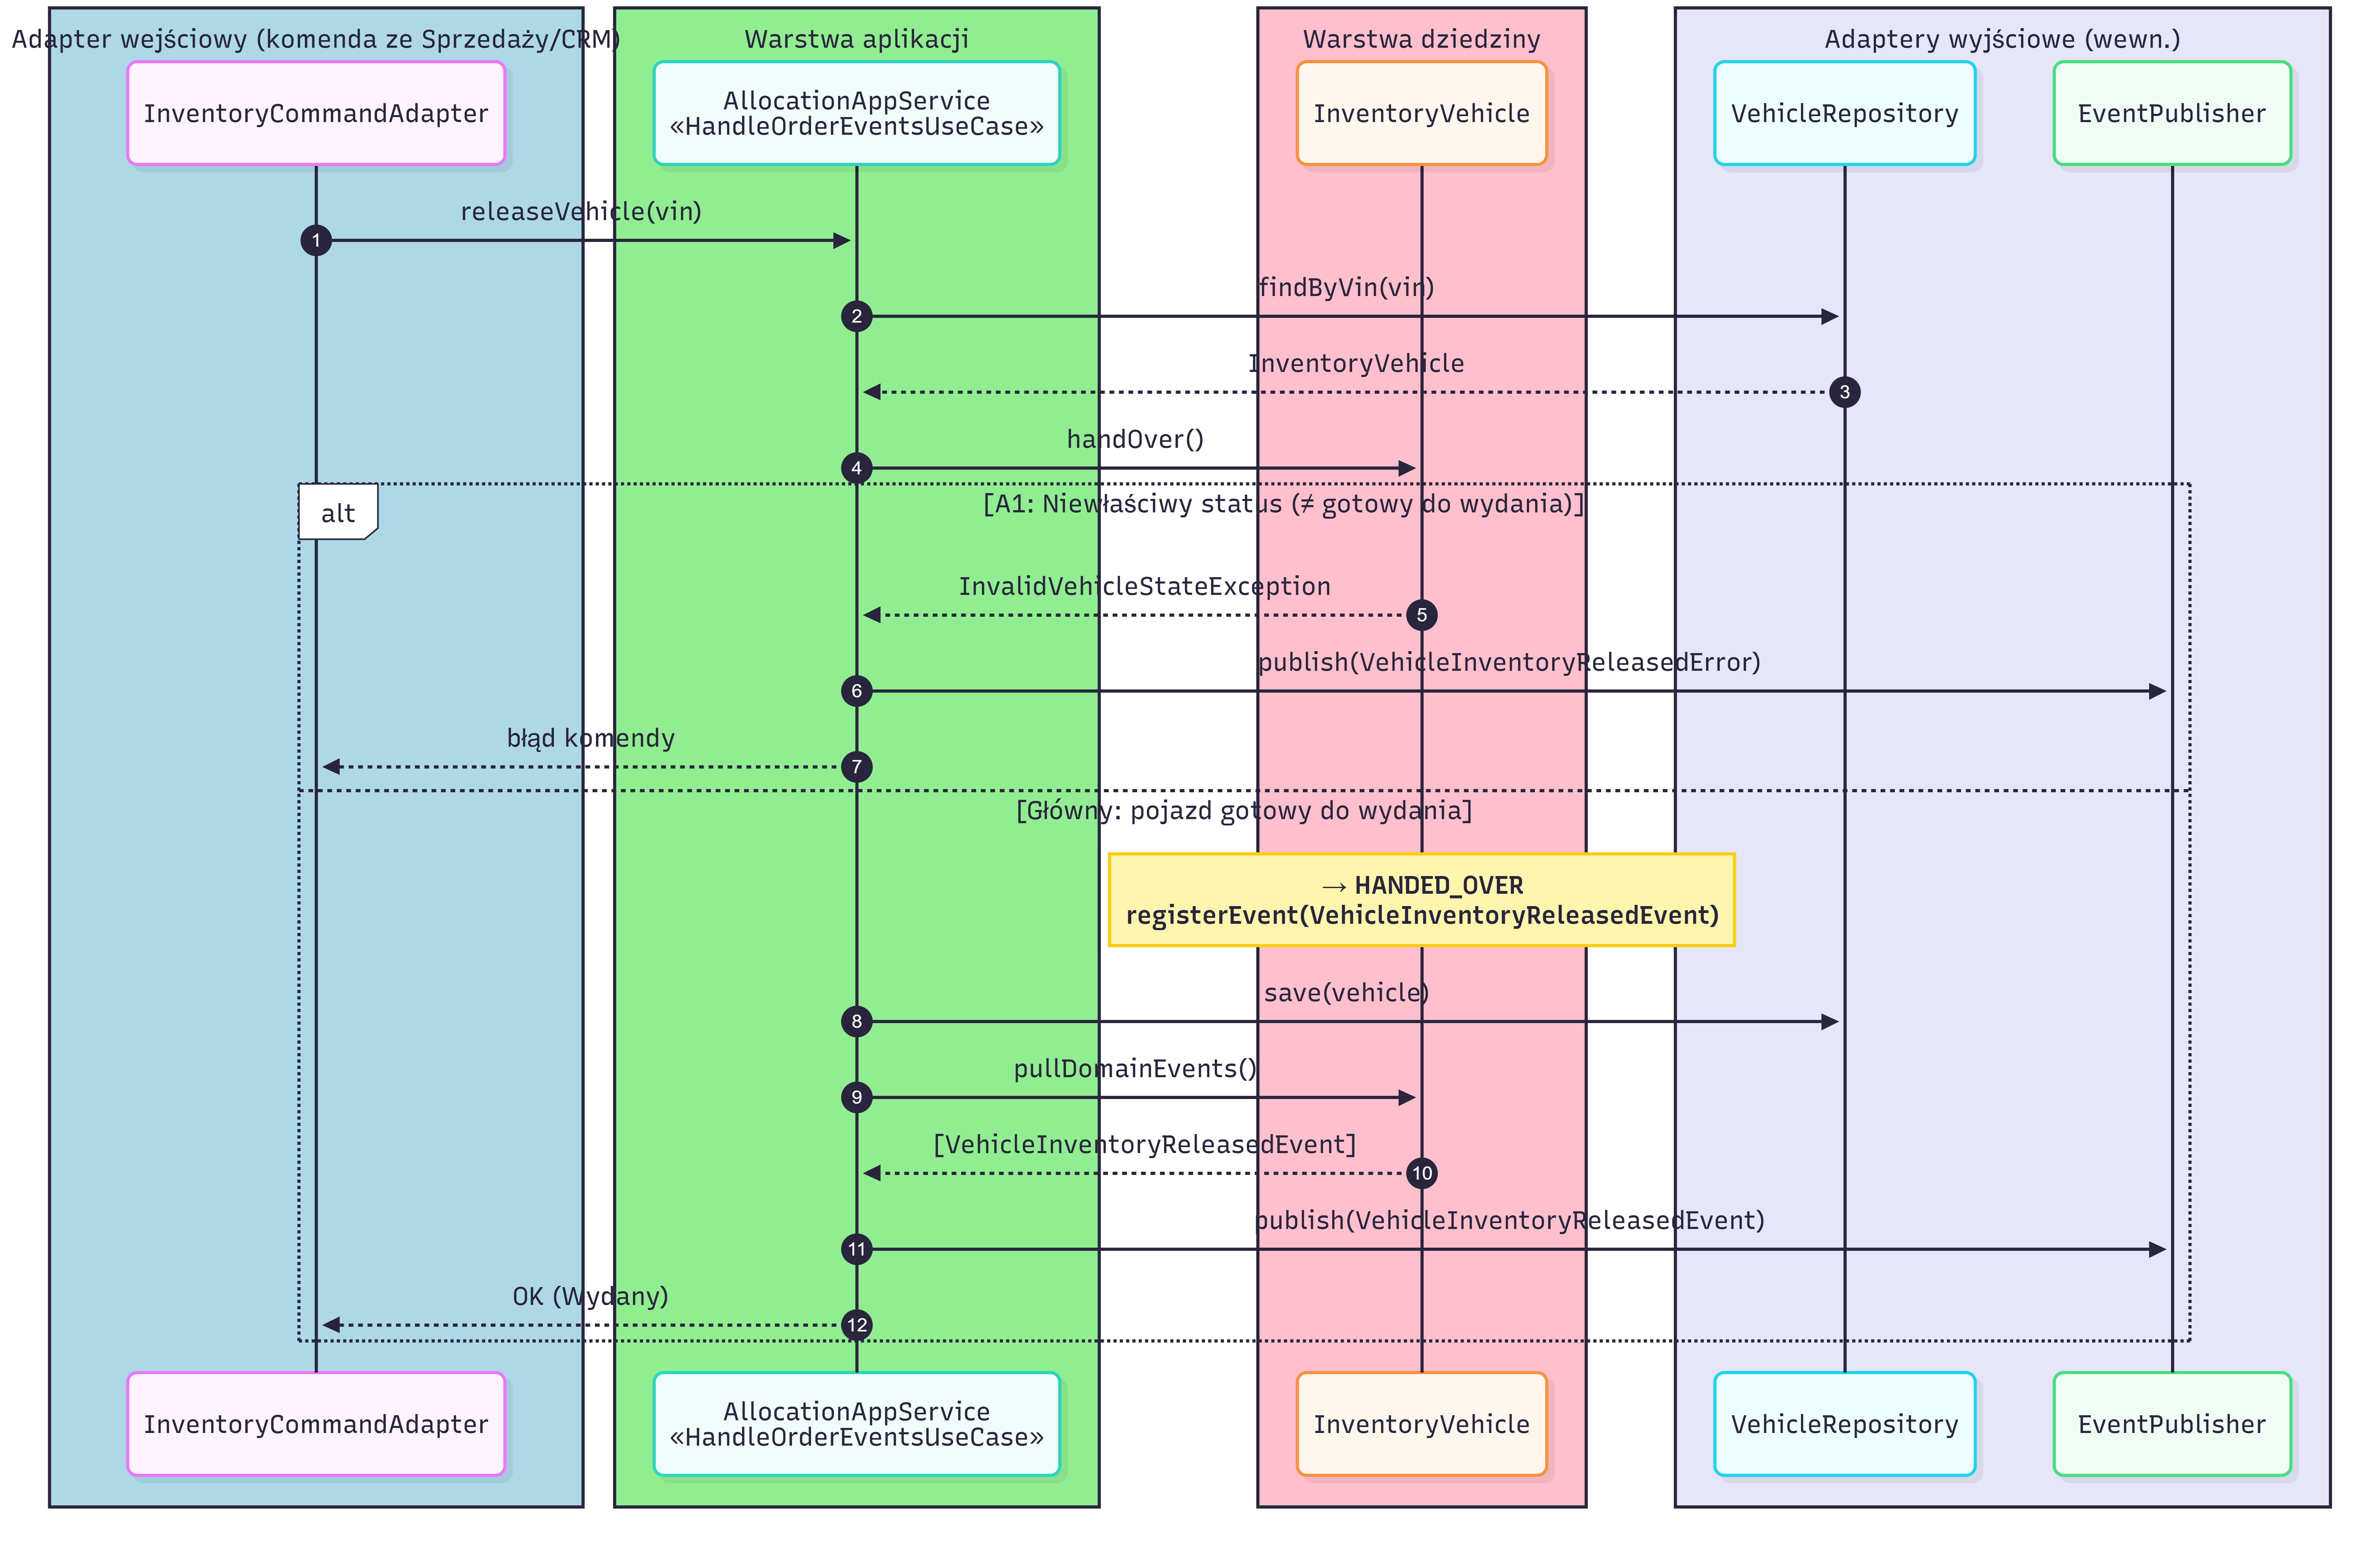
\includegraphics[width=1\textwidth]{media/diagramy_sekwencji/kontekst-inwentarza-logistyki/UC-INW-06-Sekwencji.png}
    \caption{Diagram sekwencji dla przypadku użycia UC-INW-06: Zdjęcie pojazdu ze stanu magazynowego}
    \label{fig:seq_uc_inw_06}
\end{figure}

\subsubsection{Architektura Kontekstu Inwentarza i Logistyki}

Kontekst Inwentarza i Logistyki został zaprojektowany w oparciu o architekturę heksagonalną. Diagram Architektury przedstawiono na rysunku \ref{fig:hex_logisics}.

\begin{figure}[H]
    \centering
    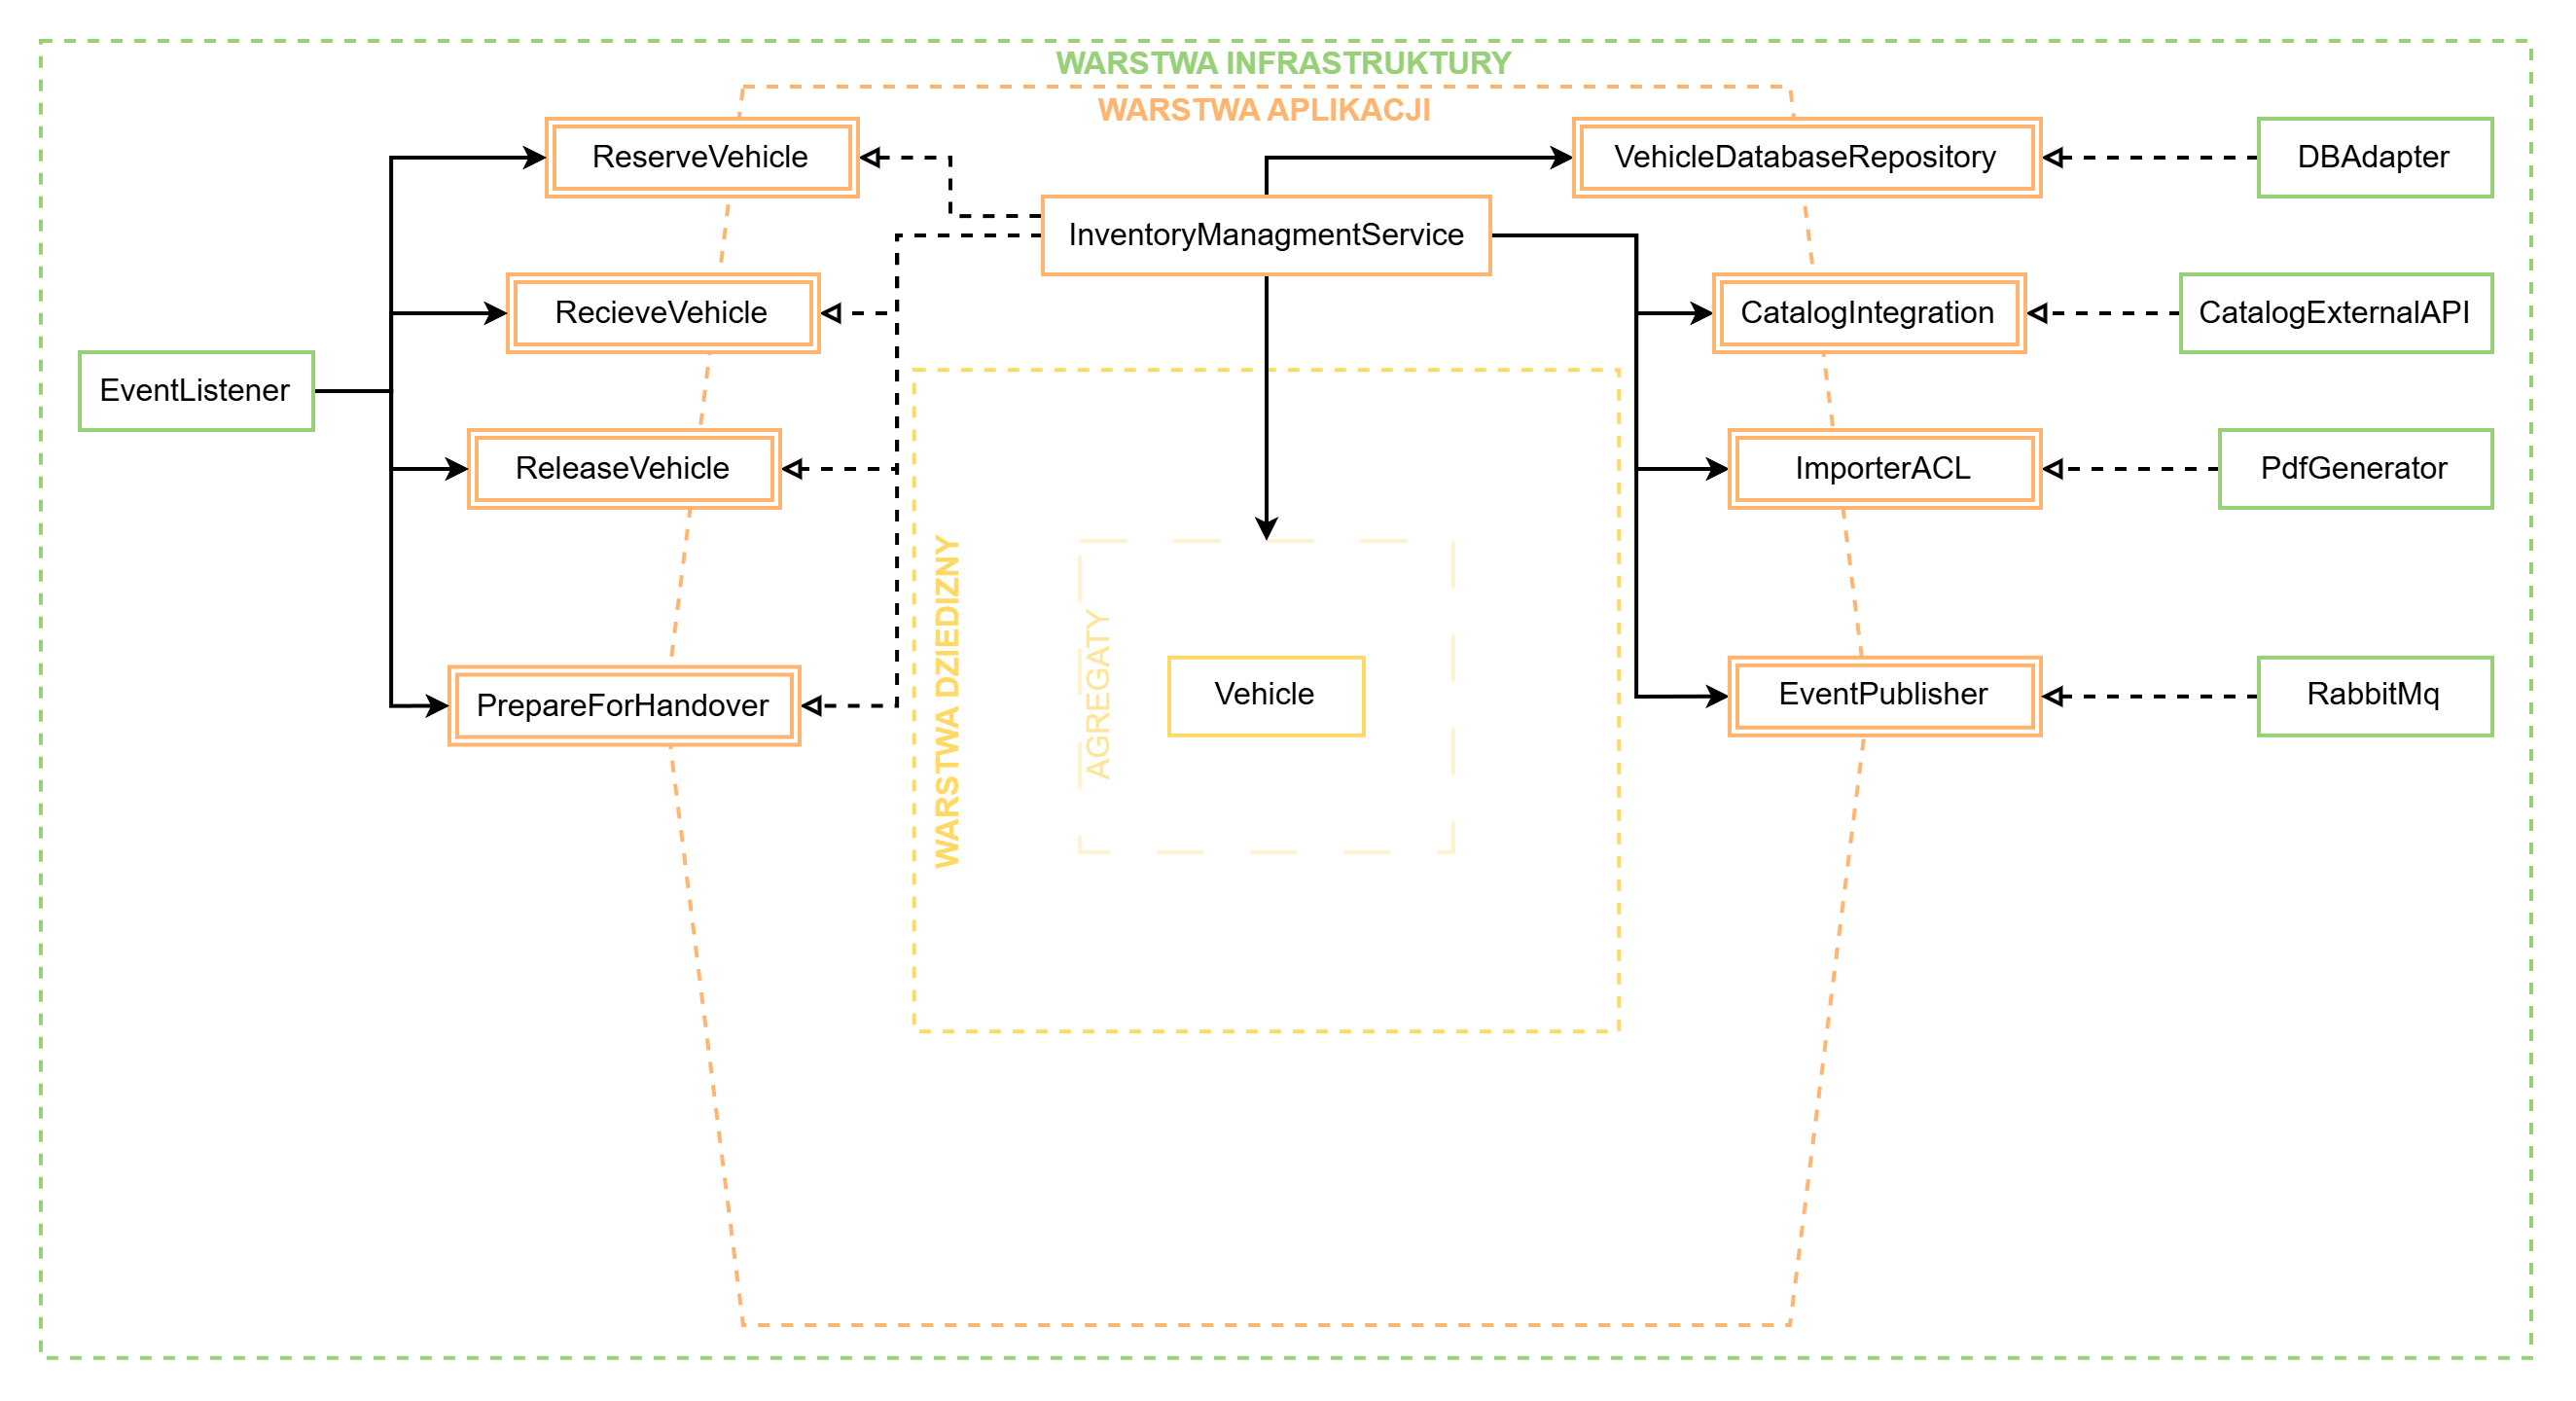
\includegraphics[width=1\linewidth]{media//architektura_heksagonalna/LogisticsArchitecture.png}
    \caption{Architektura heksagonalna kontekstu inwentarza i logistyki}
    \label{fig:hex_logisics}
\end{figure}

Poniżej przedstawiono szczegółowy opis interakcji pomiędzy warstwami, z podziałem na strony wejściową i wyjściową.

\paragraph{Strona Wejściowa: Porty i Adaptery} 
Ta strona heksagonu definiuje, w jaki sposób systemy zewnętrzne oraz operatorzy komunikują się z modułem logistyki w celu zmiany stanu magazynowego pojazdów.

Wszystkie cztery porty wejściowe realizowane są przez jedną scentralizowaną usługę \texttt{InventoryManagementService}.

\begin{itemize}
    \item \textbf{Rezerwacje i Produkcja (Asynchroniczne)}
    \begin{itemize}
        \item \textbf{Porty:} \texttt{ReserveVehicle} (UC-INW-01: rezerwacja z placu oraz UC-INW-02: zlecenie produkcji — \texttt{orderVehicleFromFactory}) i \texttt{ReleaseVehicle} (UC-INW-04: zwolnienie rezerwacji oraz UC-INW-06: zwolnienie pojazdu).
        \item \textbf{Adaptery (Messaging):} \texttt{SalesEventSubscriberAdapter} (zdarzenie \texttt{OrderPlaced} oraz komenda zwolnienia z Inwentarza), \texttt{BillingEventSubscriberAdapter} (\texttt{AdvancePaymentRegistered}~$\rightarrow$~zlecenie produkcji, \texttt{PaymentDeadlineExpired}~$\rightarrow$~zwolnienie rezerwacji), \texttt{FinancingEventSubscriberAdapter} (decyzja banku) oraz \texttt{CatalogEventSubscriberAdapter} (\texttt{SpecificationCompleted} zasilające lokalną kopię danych Katalogu).
    \end{itemize}

    \item \textbf{Obrót Magazynowy i Wydanie}
    \begin{itemize}
        \item \textbf{Porty:} \texttt{ReceiveVehicle} (UC-INW-03: przyjęcie pojazdu na plac) oraz \texttt{PrepareForHandover} (UC-INW-05: przygotowanie do wydania).
        \item \textbf{Adapter (HTTP):} \texttt{VehicleArrivalRestAdapter}. Udostępnia API dla pracowników placu, parsując żądania sieciowe o przyjęciu pojazdu na komendy wewnątrzsystemowe. Przygotowanie do wydania jest dodatkowo wyzwalane zdarzeniem \texttt{SettlementCompleted} (przez \texttt{BillingEventSubscriberAdapter}).
    \end{itemize}
\end{itemize}

\paragraph{Strona Wyjściowa: Porty i Adaptery} 
Ta strona heksagonu definiuje, czego aplikacja logistyczna potrzebuje od infrastruktury i innych modułów, aby spójnie zrealizować swoje procesy.

\begin{itemize}
    \item \textbf{Utrwalanie Stanu (Persystencja)}
    \begin{itemize}
        \item \textbf{Port:} \texttt{VehicleDatabaseRepository}. Umożliwia zapis i odczyt agregatu \texttt{InventoryVehicle}.
        \item \textbf{Adapter:} \texttt{InMemoryInventoryRepository} (węzeł \texttt{DBAdapter}). W bieżącej implementacji atrapa w pamięci; docelowo adapter bazodanowy (ORM/Hibernate) bez zmiany kontraktu portu.
    \end{itemize}

    \item \textbf{Lokalna Kopia Danych Katalogu (Read Model)}
    \begin{itemize}
        \item \textbf{Port:} \texttt{CatalogIntegration}. Zamiast synchronicznego odpytywania innych kontekstów, kontekst utrzymuje lokalną kopię danych specyfikacji, zasilaną asynchronicznie zdarzeniami (\texttt{SpecificationCompleted}, \texttt{OrderPlaced}).
        \item \textbf{Adapter:} \texttt{InMemorySpecificationReadModelAdapter}. Lokalny read model dostarczający kody wyposażenia bez sprzężenia czasowego z Katalogiem/Sprzedażą.
    \end{itemize}

    \item \textbf{Zlecanie Produkcji w Fabryce (Anti-Corruption Layer)}
    \begin{itemize}
        \item \textbf{Port:} \texttt{ImporterACL}. Port zarządzający komunikacją z systemem producenta/importera (zlecenie produkcji).
        \item \textbf{Adapter:} \texttt{FactoryIntegrationMockAdapter}. Atrapa tłumacząca żądania na format API fabryki; docelowo adapter HTTP chroniący domenę przed zmianami schematów u dostawcy.
    \end{itemize}

    \item \textbf{Publikacja Zdarzeń (Event Driven)}
    \begin{itemize}
        \item \textbf{Port:} \texttt{EventPublisher} (port Wspólnego Jądra). Umożliwia publikację zdarzeń wynikowych na magistralę.
        \item \textbf{Adapter:} \texttt{RabbitMqEventPublisherAdapter} (Wspólne Jądro). Serializuje zdarzenia dziedzinowe (np. \texttt{VehicleReservedFromStockEvent}, \texttt{VehicleReadyForHandoverEvent}, \texttt{VehicleIsNotOnStockEvent}) i wysyła je na magistralę, domykając cykl operacji logistycznych.
    \end{itemize}
\end{itemize}

\paragraph{Usługi Aplikacji}
W celu zapobiegania rozproszeniu logiki zarządzania pojazdem, wdrożono jeden centralny orkiestrator:
\begin{itemize}
    \item \textbf{InventoryManagementService} – scentralizowana usługa spinająca wszystkie przypadki użycia od UC-INW-01 do UC-INW-06. Gwarantuje jednolity punkt wejścia do mutacji stanu magazynowego. W zależności od wywołanego portu pobiera agregat \texttt{InventoryVehicle}, deleguje do niego żądania zmiany statusu, odpytuje porty wyjściowe (lokalny read model Katalogu, ACL fabryki) i utrwala wynik przez \texttt{VehicleDatabaseRepository}.
\end{itemize}

\subsubsection{Agregaty Kontekstu Inwentarza i Logistyki}

Podział na pojazdy fizycznie istniejące na placu oraz te będące jedynie wpisem w systemie fabryki podyktował wyodrębnienie jednego agregatu.

\paragraph{Agregat: Fizyczny Egzemplarz Pojazdu (\texttt{InventoryVehicle})}

% MIEJSCE NA DIAGRAM KLAS: InventoryVehicle
\begin{figure}[h]
    \centering
    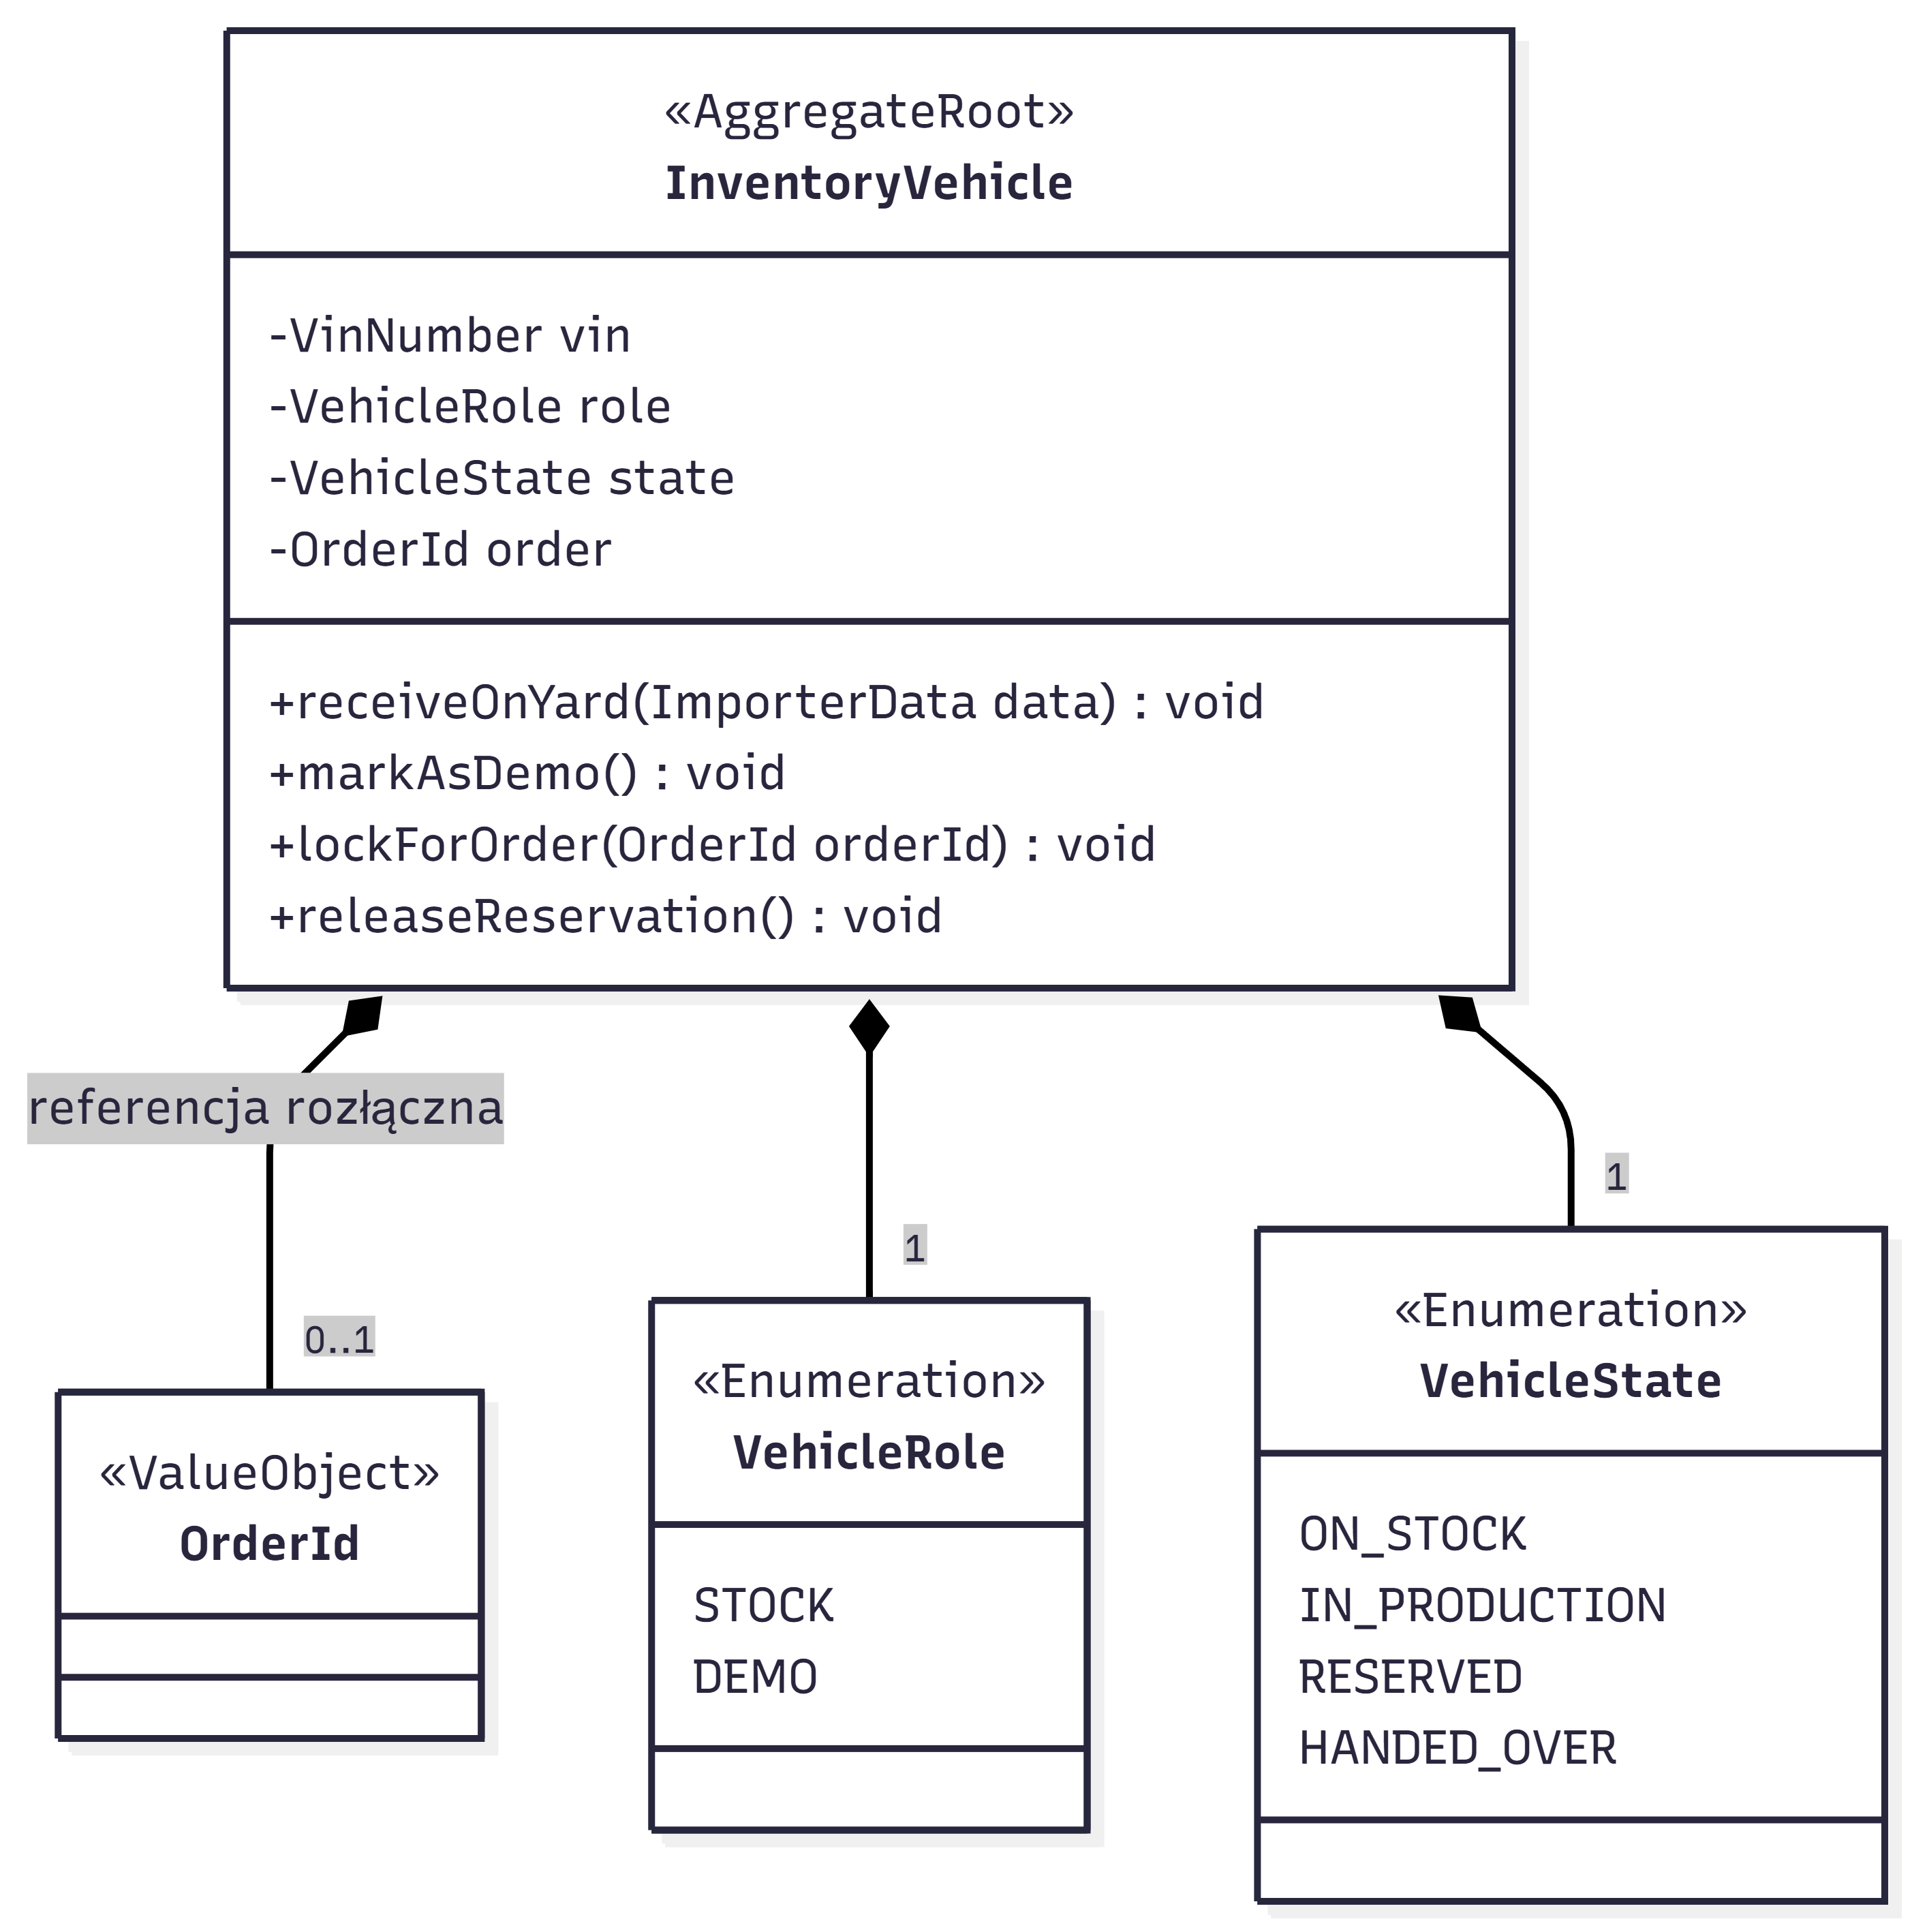
\includegraphics[width=0.5\textwidth]{media/agregaty/kontekst-inwentarza-logistyki/inventory-vehicle.png}
    \caption{Model strukturalny agregatu Fizycznego Egzemplarza Pojazdu}
    \label{fig:agg_vehicle}
\end{figure}

\paragraph{Agregat: Pojazd Magazynowy (InventoryVehicle)}
Stanowi centralny i jedyny korzeń agregatu (Aggregate Root) w Kontekście Inwentarza i Logistyki. Reprezentuje on cykl życia pojazdu w ekosystemie dealera – łącząc fazę wirtualną (zamówienie w produkcji) z fazą fizyczną (obecność na placu magazynowym). Odpowiada za utrzymanie integralności danych logistycznych i zapobieganie konfliktom rezerwacji.

\begin{itemize}
    \item \textbf{Rygorystyczna Maszyna Stanów (State Machine):} Cykl życia pojazdu kontrolowany jest przez wewnętrzną enumerację \texttt{VehicleState}. Agregat kategorycznie chroni przejścia między stanami (\texttt{IN\_PRODUCTION}, \texttt{ON\_STOCK}, \texttt{RESERVED}, \texttt{HANDED\_OVER}). Mutacje stanu odbywają się wyłącznie poprzez wysoce ekspresywne metody biznesowe. Przykładowo, metoda \texttt{receiveOnYard()} transformuje wirtualne auto z fabryki w fizyczny zasób na placu, a metoda \texttt{lockForOrder()} zmienia status na zarezerwowany.
    \item \textbf{Referencja Rozłączna i Ochrona Rezerwacji:} Powiązanie fizycznego auta z umową sprzedażową realizowane jest poprzez opcjonalny obiekt wartości \texttt{OrderId} (krotność 0..1). Agregat implementuje wzorzec twardej blokady (Pessimistic/Optimistic Locking na poziomie domeny) – metoda \texttt{lockForOrder()} hermetyzuje przypisanie zamówienia do numeru VIN, uniemożliwiając tzw. \textit{double-booking} (sprzedaż tego samego auta dwóm klientom). W przypadku zerwania umowy, metoda \texttt{releaseReservation()} czyści referencję, przywracając pojazd do wolnej puli.
    \item \textbf{Polityka Przeznaczenia (\texttt{VehicleRole}):} Aby uniknąć tworzenia nadmiarowych podklas (np. \texttt{DemoVehicle}, \texttt{StockVehicle}), agregat wykorzystuje kompozycję z enumeracją \texttt{VehicleRole}. Dzięki metodzie \texttt{markAsDemo()}, system może w dowolnym momencie wykluczyć pojazd ze standardowej puli sprzedażowej i przeznaczyć go do jazd testowych, zachowując pełną historię jego numeru VIN.
    \item \textbf{Globalna Tożsamość:} Podstawowym identyfikatorem agregatu w późniejszych fazach cyklu życia jest obiekt wartości \texttt{VinNumber}. Gwarantuje on unikalność zasobu i stanowi naturalny klucz integracyjny dla logistyki placowej (np. podczas skanowania zjazdów z lawety w procesie UC-INW-03).
\end{itemize}